% Tento soubor nahraďte vlastním souborem s obsahem práce.
%=========================================================================
% Autoři: Michal Bidlo, Bohuslav Křena, Jaroslav Dytrych, Petr Veigend a Adam Herout 2019
\chapter{Úvod}
\label{chapter:uvod}
Nejprve je nutné poznamenat, že zadání práce bylo velice obecné. Na zadání \enquote{Simulace kapalin na GPU} může být aplikováno mnoho řešení, a to nejen v~rámci modelovaného fenoménu, ale i použitých technologií a metod. Lze například simulovat jednoduchou scénu padajícího objemu dané kapaliny. Další možností je například simulace interakce mezi dvěma druhy kapalin. Bylo by i možné vytvořit systém eroze, kdy by kapalina deformovala a ničila podloží a obecně pevná tělesa vyskytující se v systému. Další možností simulace je zaměřit se detailněji na konkrétní fyzikální vlastností kapalin, jako je například adheze či povrchové napětí. Zároveň je dostupných mnoho metod jak k~simulaci přistoupit. Lze využít mřížkové metody počítající hodnoty v~předem definovaných místech, či redukovat paměťovou náročnost a využít řídkých mřížek. Možností je i využití celulárních automatů pro velmi jednoduché simulace, či využít například částicového přístupu pro mnohem složitější a fyzikálně přesnější simulace.

Tato práce se nejvíce zaměřovala na modelování fyzikálních vlastností kapalin. Přesněji řečeno se jedná o~simulaci vypařování. V~celém systému jsou jasně odlišitelné jednotlivé fáze a kapalina v~závislosti na teplotě měla plynule přechází ze skupenstvím kapalného do plynného. V~systému se zobrazuje jasná hladina s~kapalinou, její výpary pokud dochází k vypařování. Co se týče použitých metod, jsou v~práci zastoupeny dva hlavní přístupy pro modelování toku kapalin či plynů. Pro simulaci kapaliny je využito částicového přístupu, přesněji metody Smoothed Particle Hydrodynamics představené autory Monaghan \cite{Monaghan77} a Lucy \cite{Lucy77}. Pro simulaci plynného skupenství je pak využito mřížkové metody představené v~roce 1999 autorem Jos Stamem \cite{Stam99}. Aby docházelo ke správnému přenosu informací mezi jednotlivými systémy, bylo nutné následně propojit obě metody mezi sebou.

Představovaný systém lze pak využít například při demonstraci daného jevu studentům a ukázání chování kapaliny v~různých situacích. Nicméně hlavním cílem této práce je nejen vytvořit daný systém, ale především prozkoumat možnosti simulace kapalin. Primárním cílem tedy bylo prozkoumat různé metody modelování kapalin a tyto poznatky následně uplatnit při tvorbě samotné aplikace, čehož bylo docíleno  zvolením článku \cite{Evap&Cond} autorů Hendrika Hochstettera a Andrease Kolba z~University of Siegen v~Německu, zabývajícího se kondenzací a vypařováním a využívající dvě různé metody simulace.


\chapter{Teorie}
Následující kapitola se věnuje vysvětlení základní teorie skrývající se za simulacemi a animacemi tekutin a plynů. Nejprve je zde obecně vysvětlen pojem simulace a animace kapalin. Dále jsou zde vysvětleny různé přístupy k~simulaci, je zde vysvětlena mřížková neboli Eulerova metoda a částicový přístup neboli Lagrangeova metoda. V~každé sekci jsou následně popsány některé významné algoritmy spadající pod jednotlivé metody.

\label{chapter:teorie}
\section{Simulace kapalin}
Nejprve je nutné odlišit pojmy simulace kapalin a animace kapalin. V~obou případech jde především o~chování kapaliny v~určité situaci, nicméně animace se oproti simulaci zaměřuje především na vizuální stránku a méně na fyzikální přesnost. Jedná se tedy pouze o~aproximaci vzorců popisujících chování kapalin například zanedbáním velké části objemu kapaliny a popisem pouze chování hladiny kapaliny (viz obrázek \ref{fig:SWE}). Jedním z~možných využití takových aproximací jsou případy, kde natolik nezáleží na přesnosti chování, jako spíše na vizuální stránce. Příkladem mohou být videohry, ve kterých je nutné mít vizuálně přívětivou kapalinu, ale zároveň vypočitatelnou v~reálném čase s~přihlédnutím na výpočet mnoha dalších jevů v~rámci herního enginu. Avšak například při tvorbě animací a vizuálních efektů pro filmy, kde nejsme omezeni časem, lze využívat mnohem výpočetně náročnějších postupů. Tyto animace sice stále nemusí být fyzikálně dokonalé, jedná se však o~mnohem propracovanější vyobrazení kapalin, než pouhé vlnění hladiny. \cite{Medvecky-Heretik2018thesis}

\begin{figure*}[h]\centering
	\centering
	\captionsetup{justification=centering}
	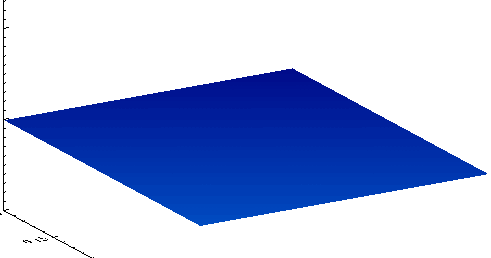
\includegraphics[width=0.3\linewidth]{obrazky-figures/SurfaceWaves/SurfWave_01.png}\hfill
	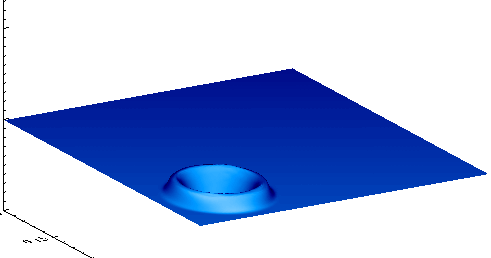
\includegraphics[width=0.3\linewidth]{obrazky-figures/SurfaceWaves/SurfWave_02.png}\hfill
	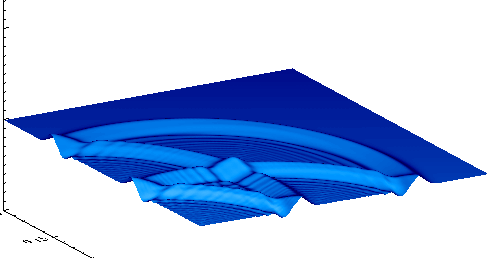
\includegraphics[width=0.3\linewidth]{obrazky-figures/SurfaceWaves/SurfWave_03.png}\hfill
	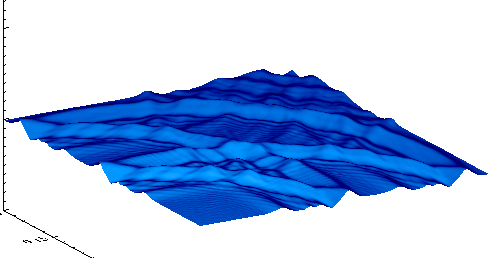
\includegraphics[width=0.3\linewidth]{obrazky-figures/SurfaceWaves/SurfWave_04.png}\hfill
	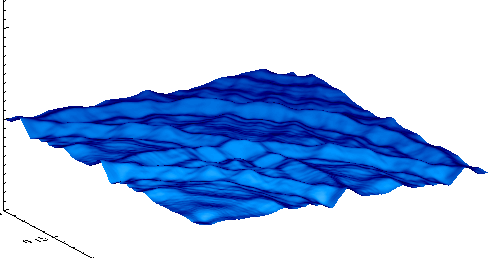
\includegraphics[width=0.3\linewidth]{obrazky-figures/SurfaceWaves/SurfWave_05.png}\hfill
	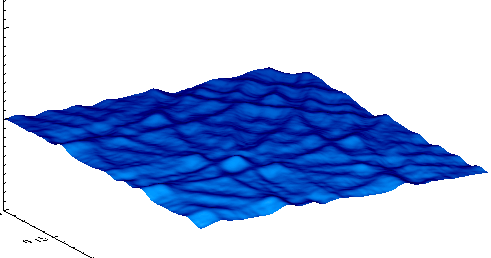
\includegraphics[width=0.3\linewidth]{obrazky-figures/SurfaceWaves/SurfWave_06.png}\hfill
	\caption{\textbf{Shallow Water Equation.} Postupné šíření vln při několika kapkách vody.}
	\textbf{Zdroj: } \url{https://en.wikipedia.org/wiki/Shallow_water_equations}
	\label{fig:SWE}
\end{figure*}

\subsubsection{Zobrazení hladiny}
Animace vlnění hladiny je jedna z~nejjednodušších vizualizací kapaliny. Existuje samozřejmě více přístupů jak takovou animaci realizovat, mezi které patří například výškové mapy, vlnová funkce či rovnice mělké vody (Shallow Water Equation) zobrazené na obrázku \ref{fig:SWE}. Ačkoliv zmíněné přítupy produkují v~celku uspokojivé vlnění hladiny, existují v~okolním světě běžné jevy, jako například lámající se vlny, které za pomocí jednoduchých vlnových funkcí a výškových map nelze simulovat. \cite{Medvecky-Heretik2018thesis}

\begin{figure}[hbt]
	\centering
	\captionsetup{justification=centering}
	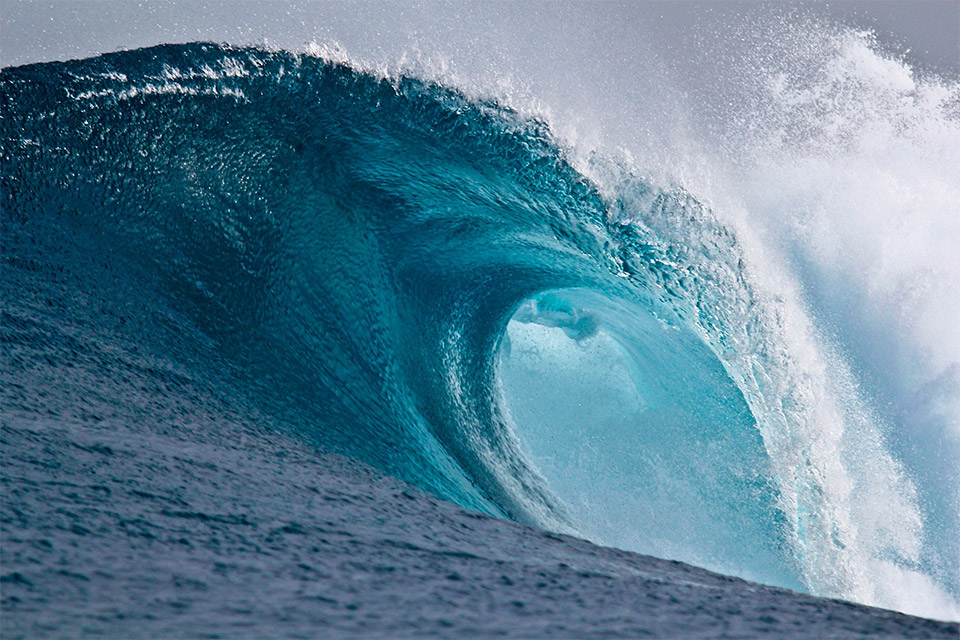
\includegraphics[width=0.4\textwidth]{obrazky-figures/Large_breaking_wave.jpg}
	\caption{\textbf{Lámající se vlna.} Jev v~reálném světě, který není realizovatelný za pomocí výškových map a vlnových funkcí.}
	\textbf{Zdroj: } \url{https://en.wikipedia.org/wiki/Breaking_wave}
	\label{keepCalm}
\end{figure}

Simulace kapalin se naopak snaží být oproti animacím co nejvíce fyzikálně přesné, čímž ale rapidně vzrůstá náročnost výpočtů. Existuje nespočet metod jak dosáhnout výsledku, nicméně čím přesnější a složitější scéna, tím delší výpočet daného scénáře. Doba výpočtu se tak může pohybovat v~rámci minut, ale i hodin. Tyto metody jsou pak často založeny nad numerickými výpočty fyzikálních rovnic, kde nejpoužívanější rovnice jsou Navier-Stokesovy rovnice.

\subsection{Navier-Stokesovy rovnice}
Navier-Stokesovy rovnice jsou jedny z~nejvyužívanějších rovnic pro výpočty chování kapalin. Základy pro popis dynamiky kapalin položil již v~roce 1687 Sir Isaac Newton v~článku "Principa", kde bylo poprvé správně popsáno chování viskózních kapalin. Později Daniel Bernoulli a Leonhard Euler popsali chování neviskózního toku pomocí rovnic dnes známých jako Eulerovy neviskózní rovnice (Euler’s inviscid equations). Až Claude-Louis Navier a Sir George Stokes na sobě nezávisle odvodili finální podobu rovnic ze zmiňovaných Eulerových a Newtonových rovnic. Tyto Navier-Stokesovy rovnice (rovnice \ref{eq:NavierStokes} a \ref{eq:NavierStokes2})  jsou nyní nejpoužívanější formou popisu chování kapalin a bylo na nich postaveno nespočet různých algoritmů. \cite{simscale_2020}

\begin{equation}
	\rho(\frac{\partial}{\partial t} + \mathbf{u} \cdot \nabla)\mathbf{u} = -\nabla p + \mu\nabla\cdot(\nabla \mathbf{u}) + f
	\label{eq:NavierStokes}
\end{equation}

\begin{equation}
	\nabla \cdot \mathbf{u} = 0
	\label{eq:NavierStokes2}
\end{equation}

Tři základní vlastnosti viskózní kapaliny, která má neměnné teplo, jsou rychlost ($\mathbf{u}$), tlak ($p$) a hustota ($\rho$). V~rovnici \ref{eq:NavierStokes} pak $\mu$ označuje viskozitu kapaliny a $f$ ostatní síly působící na kapalinu, jako například gravitace. Tyto rovnice tudíž vyjadřují zákon o~zachování hybnosti a zákon o~zachování hmotnosti pro Newtonské kapaliny. Newtonská kapalina je kapalina kterou lze popsat lineárním Newtonovým modelem. Její viskozita je závislá především na tlaku a teplotě a z~tohoto hlediska se jedná o~takzvanou Newtonskou viskozitu. U~nenewtonské kapaliny pak popisujeme takzvanou zdánlivou viskozitu závislou na předchozí deformaci kapaliny a rychlosti vnitřního smyku kapaliny. Tyto kapaliny pak nelze popsat lineárním Newtonovým zákonem.\cite{StejskalJan2013Pmks}

Navier-Stokesovy rovnice jsou hojně využívány nejen pro simulaci a animaci kapalin, ale v~celé řadě dalších vědních oborů. Využití můžeme nalézt při vytváření modelů pro předpověď počasí, pro studování toku vzduchu při výrobě letadel nebo například při analýze šíření znečištění.
\break

Existují dva úhly pohledu na organizaci a řešení nejen těchto rovnic, ale zároveň obecně na řešení dynamiky kapalin. Tyto metody se pak liší především v~bodech pozorování. V~Eulerově metodě dochází k~výpočtu požadovaných hodnot v~přesně daných bodech, tedy v~určité diskrétní mřížce. U~Lagrangeovy metody dochází k~výpočtu v~bodech sledované masy, tedy v~částicích sledované kapaliny. Níže jsou obě metody detailněji popsány, včetně několika algoritmů, které pod dané metody spadají.

\begin{figure}[h]
	\centering
	\begin{subfigure}{.5\textwidth}
		\centering
		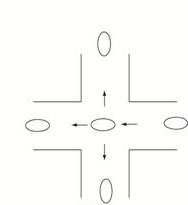
\includegraphics[width=0.7\linewidth]{obrazky-figures/EulerLagran_02.jpg}
		\caption{\textbf{Eulerův přístup}}
		\label{fig:Euler}
	\end{subfigure}%
	\begin{subfigure}{.5\textwidth}
		\centering
		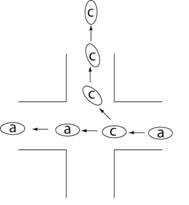
\includegraphics[width=0.7\linewidth]{obrazky-figures/EulerLagran_01.jpg}
		\caption{\textbf{Lagrangeův přístup}}
		\label{fig:Lagran}
	\end{subfigure}
	\caption{\textbf{Příklad dvou přístupů nad křižovatkou s~auty.} Eulerův přístup (\ref{fig:Euler}) sleduje křižovatku v~předem daných místech (ramena a střed křižovatky). Naopak Lagrangeův přístup(\ref{fig:Lagran}) sleduje konkrétní vozidla (a,c), jak projíždí křižovatkou.}
	\textbf{Zdroj:} \url{http://abe-research.illinois.edu/faculty/dickc/Engineering/ELdescrip2a.htm}
	\label{fig:Cross}
\end{figure}

\section{Eulerova metoda toku}
Jak bylo popsáno výše, při využití Eulerovy metody jsou vlastnosti kapaliny počítány v~pevně definovaných bodech diskrétní mřížky. Ačkoliv některé vlastnosti kapaliny popisuje Eulerova metoda mnohem přesněji, největší nevýhodou je samotná mřížka. Jeden z~prvních problémů je hrubost mřížky. Při pohledu na obrázek \ref{fig:EulerGrid} je patrné, že reálná hladina je lehce zvlněná, ale z~důvodu velké hrubosti mřížky a tedy hrubějšímu vzorkování, by lehké zvlnění bylo zanedbáno a hladina by byla rovná.

Dalším problémem je paměťová náročnost. je-li využito jemnější mřížky, z důvodu odstranění problémů souvisejících s~hrubou mřížkou, je nutno počítat se zvyšující se paměťovou náročností. Při výpočtech v trojrozměrném prostoru a s dvojnásobným zpřesněním v~každé ose, dojde k s~osminásobně zvýšenému počtu buněk v~paměti. Tento problém však naštěstí lze již řešit pomocí různých struktur jako jsou například řídké mřížky, u kterých dochází k zvýšené jemnosti pouze v potřebných oblastech.
%\todo{popis řídké mřížky}

Posledním problémem je samotná uzavřenost mřížky, která brání k~plně dynamické simulaci. Kapalina je tedy uzavřena do \enquote{nerozbitné nádoby} a jakýkoliv pokus o~její tok mimo mřížku je nemožný. I~na tento problém však existuje řešení, a to v~podobě dynamických mřížek, které se v~případě nutnosti dokáží rozšiřovat v~prostoru a poskytují tak možnosti pro rozsáhlejší simulační prostor.
\cite{KelagerSPH}

\begin{figure}[hbt]
	\centering
	\captionsetup{justification=centering}
	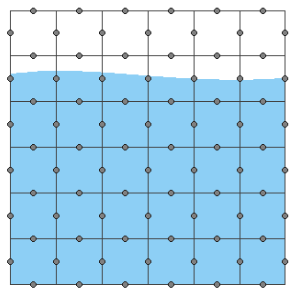
\includegraphics[width=0.4\textwidth]{obrazky-figures/GridEuler.PNG}
	\caption{\textbf{Eulerova mřížka.} Kapalina uzavřená ve 2D mřížce. Rychlost a ostatní vlastnosti kapaliny jsou reprezentovány pouze ve vyznačených tečkách. Z důvodu hrubosti mřížky, pak může docházet k zanedbání některých detailů.}
	\textbf{Zdroj: } Lagrangian Fluid Dynamics Using Smoothed Particle Hydrodynamics \cite{KelagerSPH}
	\label{fig:EulerGrid}
\end{figure}

\subsection{Mřížková metoda}
\label{chapter:Grid}
Mřížková (Grid) metoda je Eulerovská metoda využívající pro pohyb kapaliny několika polí vektorů. Základem mřížkové metody je pole vektorů rychlostí pro každý zkoumaný bod v~mřížce. Toto pole pak představuje pohyb tekutiny v~celém zkoumaném prostoru. Toto pole lze vyjádřit rovnicí \ref{eq:velocityField}
\begin{equation}
	\Vec{u}(x,y) = (u_x,u_y)
	\label{eq:velocityField}
\end{equation}

\begin{figure}[hbt]
	\centering
	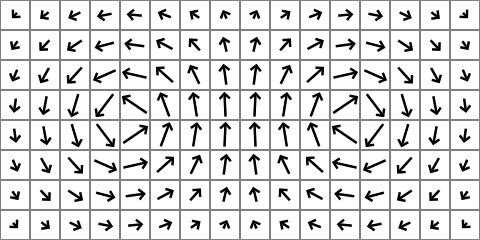
\includegraphics[width=0.45\textwidth]{obrazky-figures/flow-field.png}
	\caption{\textbf{Pole rychlostí.} Šipky v~poli označují velikost a směr proudění.}
	\textbf{Zdroj: } \url{https://www.karlsims.com/fluid-flow.html}
	\label{fig:VelocityField}
\end{figure}

Dalším základním stavebním kamenem algoritmu je pak advekce, neboli přesun vlastností z~jednoho místa na jiné v~důsledku pohybu kapaliny. Je li uvažováno, že tok kapaliny přenáší například určitou koncentraci částic (kouř, barvivo, písek), pak existují dvě možnosti jak posunout dané hodnoty v~čase a prostoru.  První možností je dopředný posun v~čase vyjádřen rovnicí \ref{eq:fwdAdvection}. V~závislosti na pozici $\mathbf{r}$ v prostoru je zvolena odpovídající rychlost $\mathbf{u}$ a danou hodnota $A$ je posunuta v~prostoru.

\begin{equation}
	A(\mathbf{r} + \mathbf{u}\Delta t, t + \Delta t) = A(\mathbf{r}, t)
	\label{eq:fwdAdvection}
\end{equation}

Druhým možným přístupem pro přesun hodnot je tzv. backtracking. V~tomto přístupu není hodnota posunuta z~jedné pozice na druhou. Vektor rychlosti se naopak invertuje a do nynější pozice se přesouvá pozice předchozí. Následující rovnice \ref{eq:backAdvection} popisuje právě tuto metodu. \cite{webglFluid}

\begin{equation}
	A(\mathbf{r}, t + \Delta t) = A(\mathbf{r} - \mathbf{u}\Delta t, t)
	\label{eq:backAdvection}
\end{equation}

\begin{figure}[h]
	\centering
	\captionsetup{justification=centering}
	\begin{subfigure}{.5\textwidth}
		\centering
		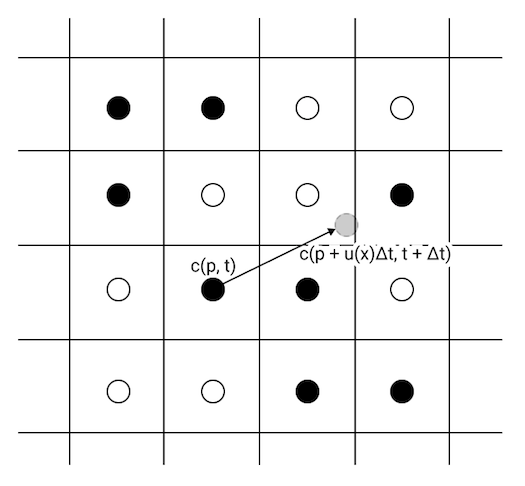
\includegraphics[width=0.5\linewidth]{obrazky-figures/advection1.png}
		\caption{\textbf{Dopředná advekce}}
		\label{fig:fwbAdvection}
	\end{subfigure}%
	\begin{subfigure}{.5\textwidth}
		\centering
		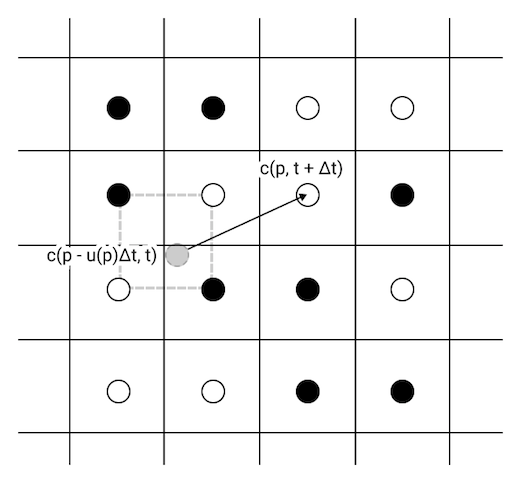
\includegraphics[width=0.5\linewidth]{obrazky-figures/advection2.png}
		\caption{\textbf{Zpětná advekce}}
		\label{fig:backAdvection}
	\end{subfigure}
	\caption{\textbf{Příklad dvou přístupů advekce.} Na obrázku \ref{fig:fwbAdvection} lze vidět dopředný posun hodnot, kdy je například hustota posouvána vpřed, ve směru vektoru rychlosti. Na obrázku \ref{fig:backAdvection} je následně znázorněn zpětný posun, kdy dochází k otočení vektoru rychlosti a pomocí interpolace je zjišťuje jaká hodnota \enquote{doputovala} na současnou pozici.}
	\textbf{Zdroj:} Fluid Simulation (with WebGL demo) \cite{webglFluid}
	\label{fig:advection}
\end{figure}

Stejně jako dochází k přesunu určité hodnoty v~prostoru, lze přesouvat i pole rychlostí a měnit jej tak v~čase. V~tomto případě však můžou nastat problémy s~nestlačitelností a zákonem zachování hmotnosti. Je nutné zaručit, že divergence pole rychlosti je všude nulová. Divergence zjednodušeně říká, zda v~určitém bodě daná vlastnost roste, či klesá. Pokud je vyžadováno docílit nulové divergence pole rychlosti, jedná se o docílení stavu, kde v~žádném bodě neklesá ani neroste hustota kapaliny. \cite{webglFluid}

\begin{figure}[h]
	\centering
	\begin{subfigure}{.3\textwidth}
		\centering
		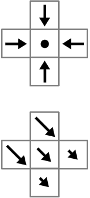
\includegraphics[width=0.35\linewidth]{obrazky-figures/div-negative.png}
		\caption{\textbf{Záporná divergence}}
		\label{fig:divPlus}
	\end{subfigure}%
	\begin{subfigure}{.3\textwidth}
		\centering
		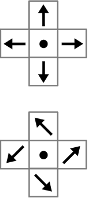
\includegraphics[width=0.35\linewidth]{obrazky-figures/div-positive.png}
		\caption{\textbf{Kladná divergence}}
		\label{fig:divNeg}
	\end{subfigure}
	\begin{subfigure}{.3\textwidth}
		\centering
		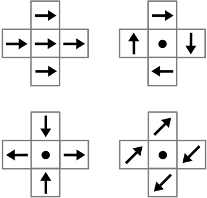
\includegraphics[width=0.8\linewidth]{obrazky-figures/div-zero.png}
		\caption{\textbf{Nulová divergence}}
		\label{fig:divZero}
	\end{subfigure}
	\caption{\textbf{Příklady divergence } Příklady různých divergencí v~bodě, v~závislosti na velikosti a směru vektorového pole v~okolí. Na obrázcích \ref{fig:divPlus} a a\ref{fig:divNeg} si lze všimnout, že v v prostřední buňce dochází k přílišnému hromadění či úbytku hodnot.}
	\textbf{Zdroj:} \url{https://www.karlsims.com/fluid-flow.html}
	\label{fig:div}
\end{figure}

Při výpočtu pole s~nulovou divergencí lze využit takzvaný Helmholtz-Hodgeův rozkladový teorém \ref{eq:HelmHodge},
\begin{equation}
	\mathbf{u} = \mathbf{w} - \nabla p
	\label{eq:HelmHodge}
\end{equation}
kde $\mathbf{u}$ je zmíněné hledané pole s~nulovou divergencí, $\mathbf{w}$ je pole rychlostí s~nenulovou divergencí a $\nabla p$ je gradient tlaku. Tato rovnice tedy říká, že pole rychlostí s~nenulovou divergencí může být opraveno pomocí gradientu tlaku. Pro výpočet tlaku lze pak odvodit ze stejného teorému \ref{eq:HelmHodge} následující rovnici \ref{eq:gridPress}. \cite{webglFluid}

\begin{equation}
	p_{x,y}^{(k+1)} = \frac{p_{x+1,y}^{(k)} + p_{x-1,y}^{(k)} + p_{x,y+1}^{(k)} + p_{x,y-1}^{(k)} + \alpha b_{x,y}}{\beta}
	\label{eq:gridPress}
\end{equation}

Přičemž pro neviskózní kapaliny platí, že v rovnici \ref{eq:gridPress} mají konstanty následující hodnoty $\alpha = -( velikost\_bunky )^2$, $\beta = 4$ a $b = \nabla \cdot \mathbf{w}$. Tato rovnice je pak řešena například Jacobiho iterativní metodou, kde počáteční odhad je nulový tlak ve všech bodech. Po dostatečném počtu iterací je výsledkem hodnota tlaku ve všech bodech a po výpočtu gradientu a aplikování ve vzorci \ref{eq:HelmHodge} je získáno pole rychlostí s~nulovou divergencí. Pomocí tohoto pole pak lze posouvat výše zmíněné hodnoty jako je barva, koncentrace částic a jiné.
\cite{GPUGemsGridFLuid}

\begin{figure}[hbt]
	\centering
	\captionsetup{justification=centering}
	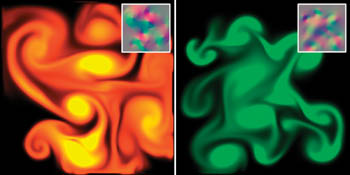
\includegraphics[width=0.5\textwidth]{obrazky-figures/GridFluid.jpg}
	\caption{\textbf{Mřížková metoda.} Vizualizace barviva v~proudícího vodě.}
	\textbf{Zdroj: } Chapter 38. Fast Fluid Dynamics Simulation on the GPU \cite{GPUGemsGridFLuid}
	\label{fig:EulerFluid}
\end{figure}

%\todo{využití, výhody/nevýhody}
\subsection{Celulární automaty}
Pro simulaci toku kapalin lze využít i celulárních automatů. Celulární automat se skládá z~několika důležitých částí, stavového prostoru rozděleného na diskrétní buňky, přechodové funkce a množiny stavů, které mohou buňky nabývat. Celulární automaty pracují na principu $n$-dimenzionálního okolí, kde $n$ závisí na dimenzi zkoumaného prostoru a typu okolí. V~jednom časovém kroku se pak aplikuje na všechny buňky přechodová funkce, která vyhodnotí stavy okolních buněk a podle výsledku nastaví vlastní stav.

\begin{figure}[hbt]
	\centering
	\captionsetup{justification=centering}
	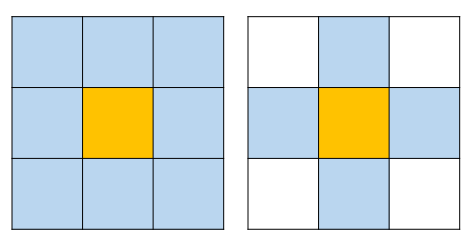
\includegraphics[width=0.5\textwidth]{obrazky-figures/Neighborhood.png}
	\caption{\textbf{Typy okolí.} Vlevo Moorovo okolí, vpravo Von-Neumanovo}
	\textbf{Zdroj: } \url{http://complextin.blogspot.com/2016/06/2d-cellular-automata-three-state.html}
	\label{fig:neighbours}
\end{figure}

Pomocí popsaného principu a využití několika jednoduchých pravidel pak lze vytvořit velice jednoduchý simulátor toku vody. Nejdříve se simuluje působení gravitace a automat se pokusí co nejvíce vody přesunout o~buňku níže. Pokud je buňka plná nebo se jedná o~buňku, do které nemůže téci voda, zbylá kapalina je distribuována do okolních horizontálních buněk. Jedná se o~velice jednoduchý algoritmus, který však zanedbává mnoho vlastností kapalin. Prvním problémem je situace při spojených nádobách, kdy pomocí tohoto algoritmu nedojde k~vyrovnání hladin a je nutné aplikovat další procesy pro vyrovnávání hladin. Dalším problémem je odrazivost a rychlost toku kapalin. Kapalina se bude vždy pohybovat stejnou rychlostí a představíme-li si situaci kdy \enquote{naráží} do stěny, pak nedojde k~roztříštění a případnému stoupání kapaliny vzhůru. Dalším problémem mohou být vlastnosti kapaliny, jako je například viskozita, která se zanedbává, případně může být simulována pouhým koeficientem ovlivňujícím rychlost toku. \cite{Medvecky-Heretik2018thesis}

\begin{figure*}[h!]\centering
	\centering
	\captionsetup{justification=centering}
	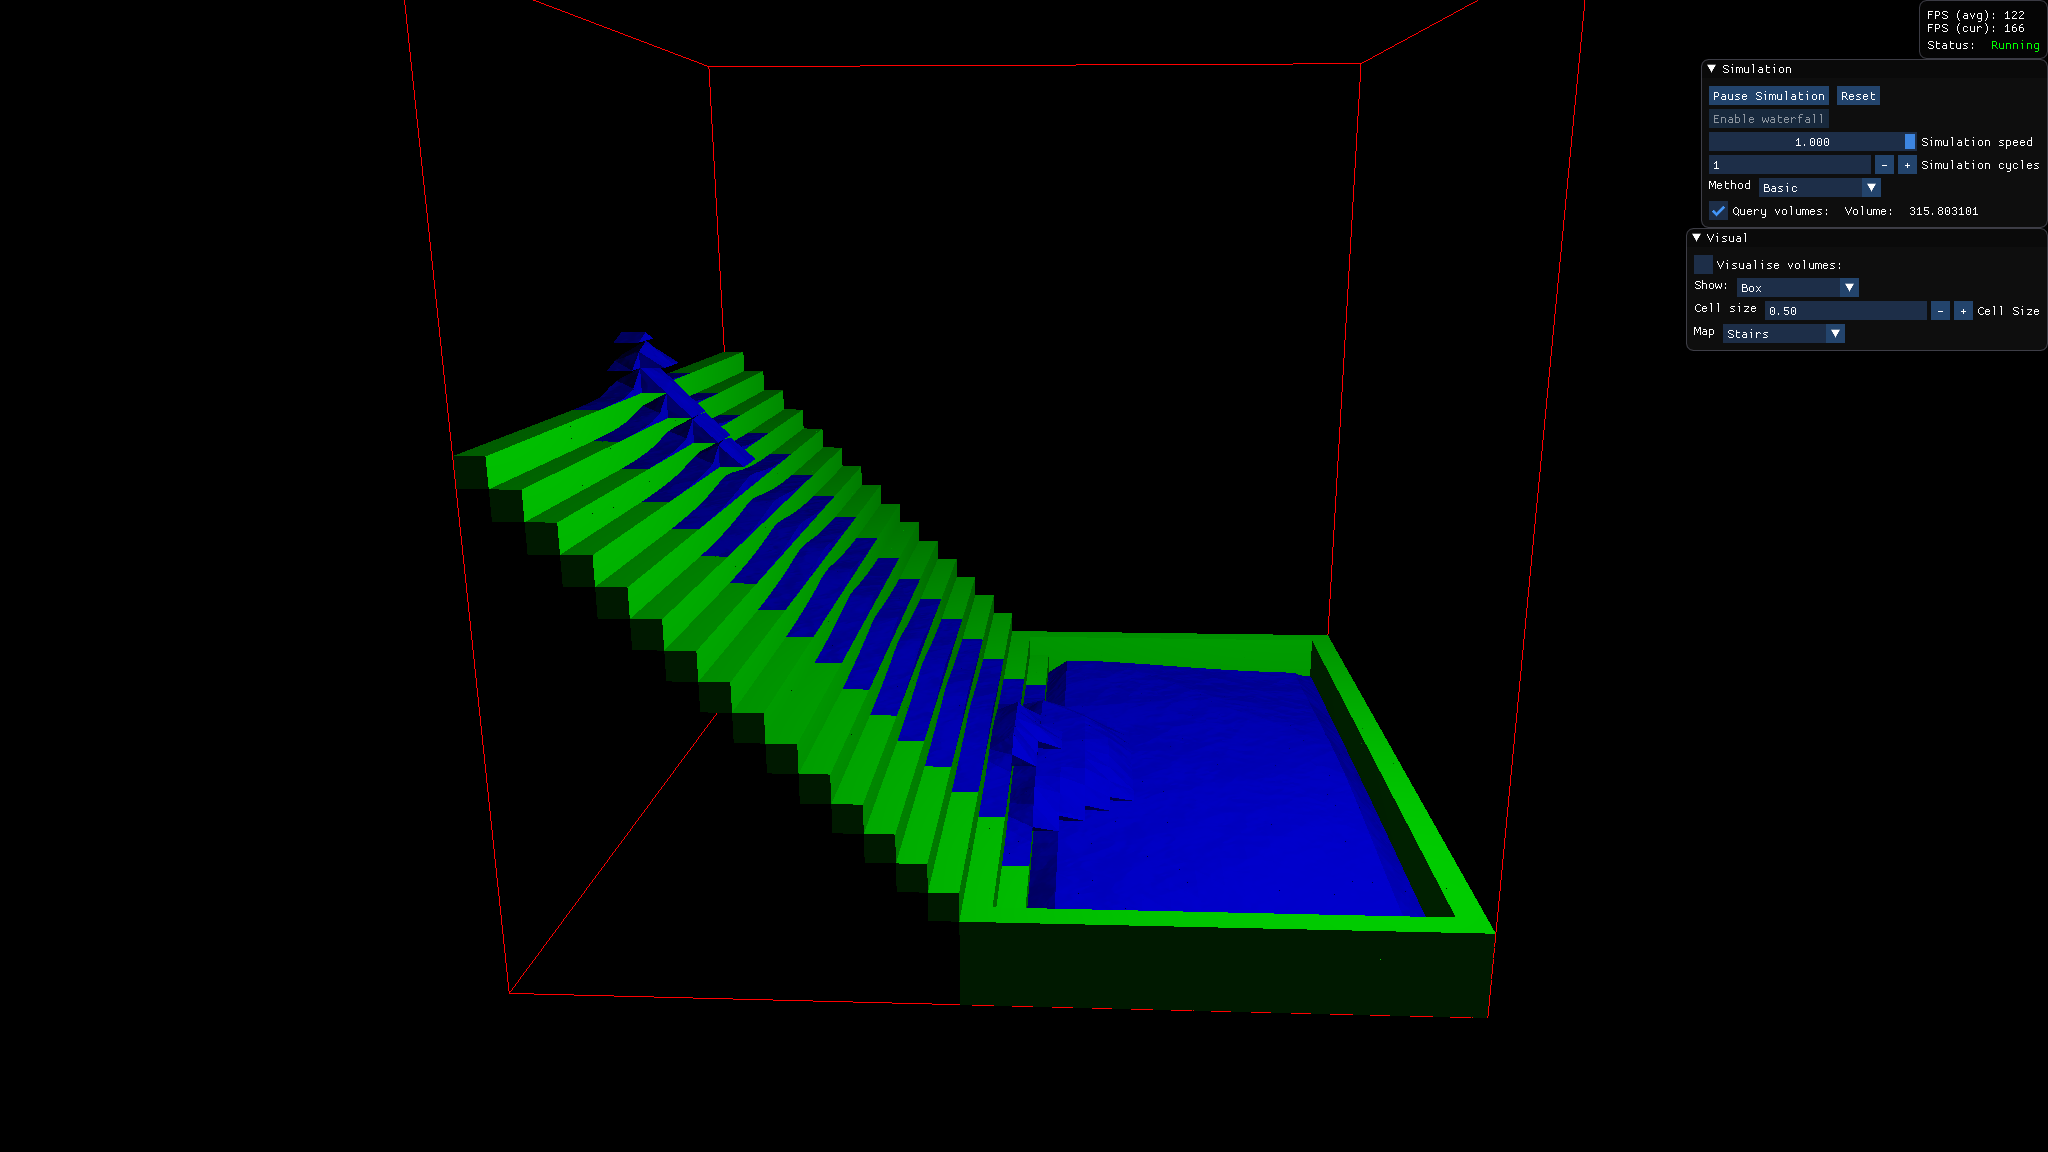
\includegraphics[width=0.5\linewidth]{obrazky-figures/cellular1.png}\hfill
	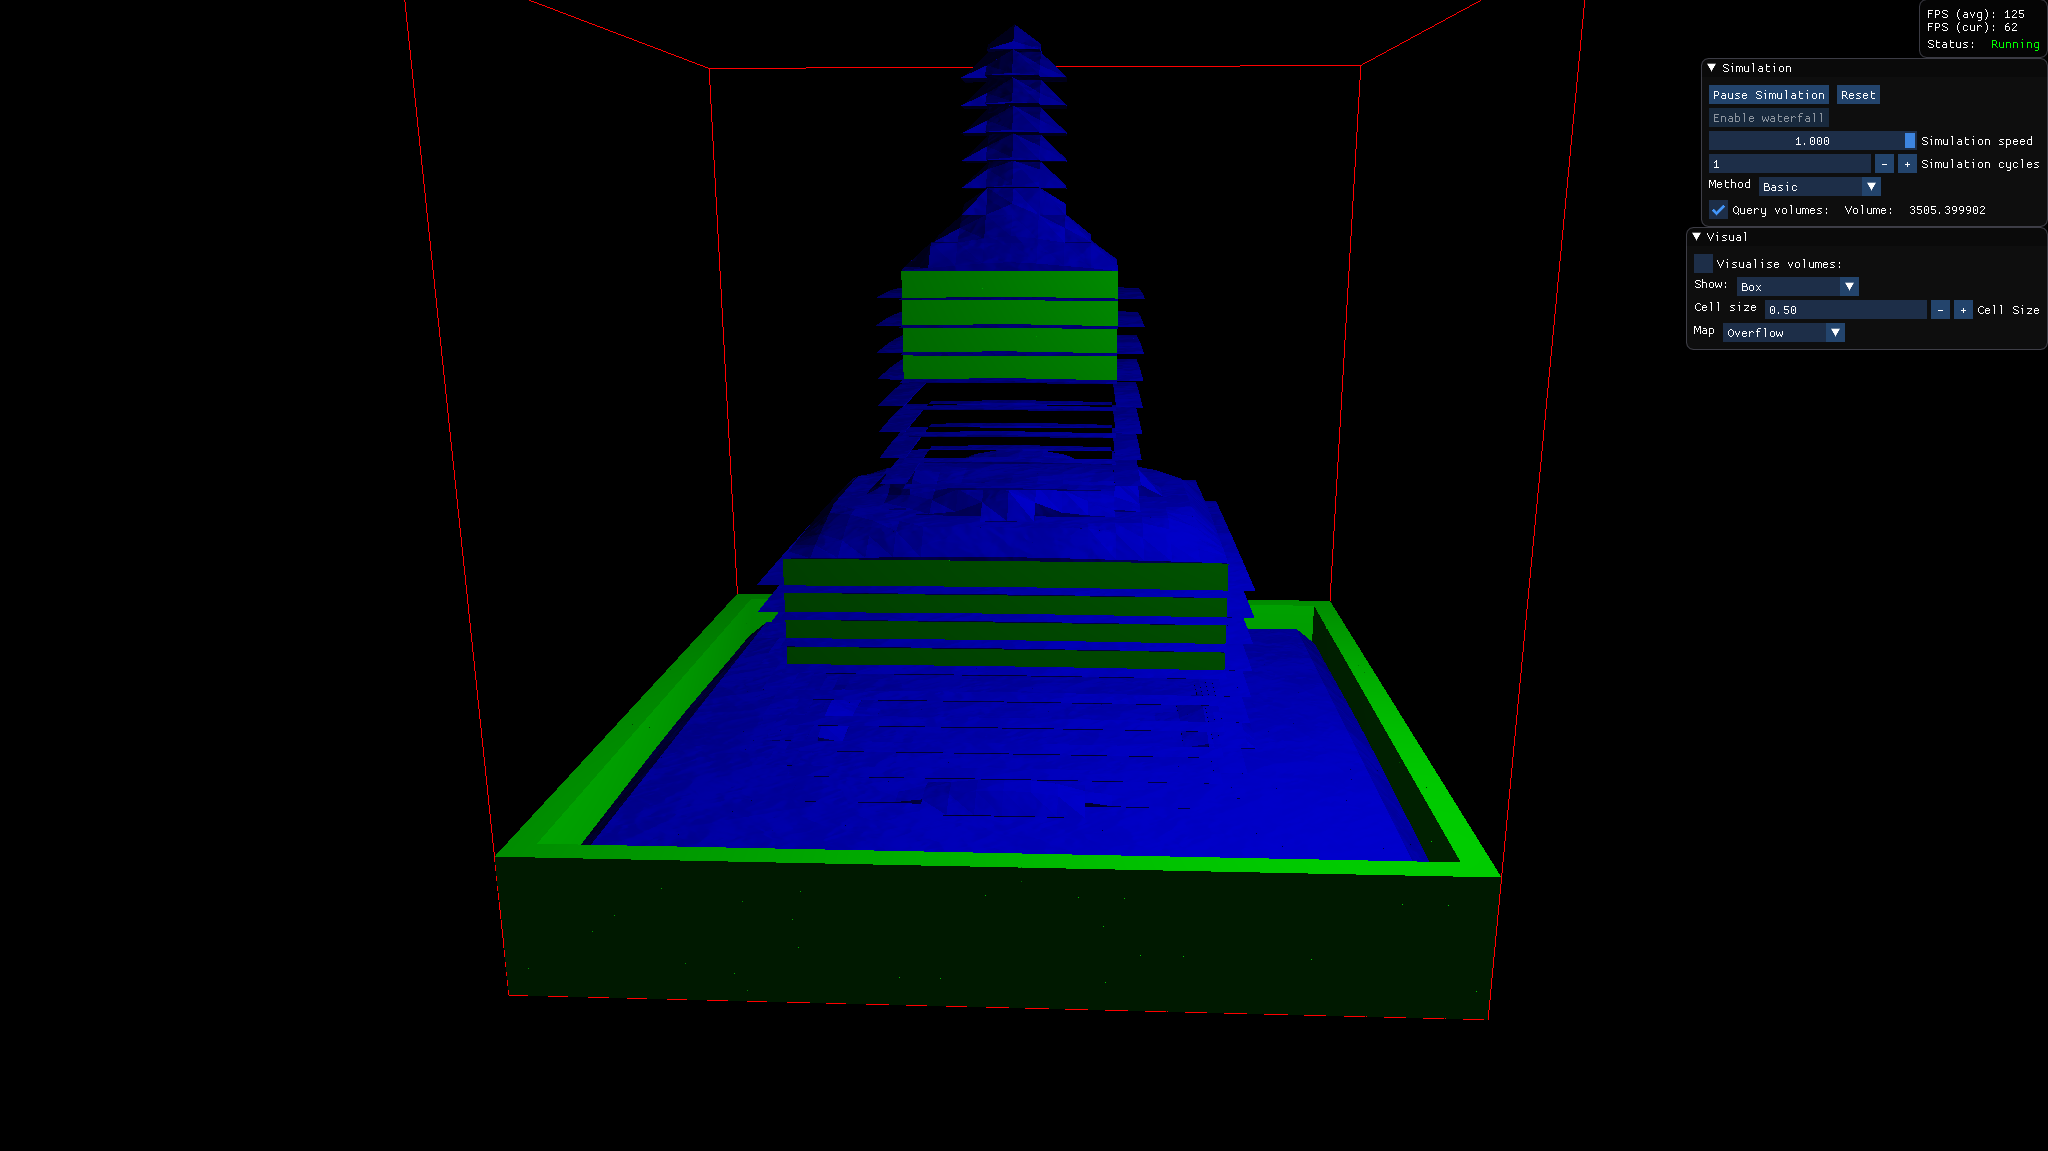
\includegraphics[width=0.5\linewidth]{obrazky-figures/cellular2.png}\hfill
	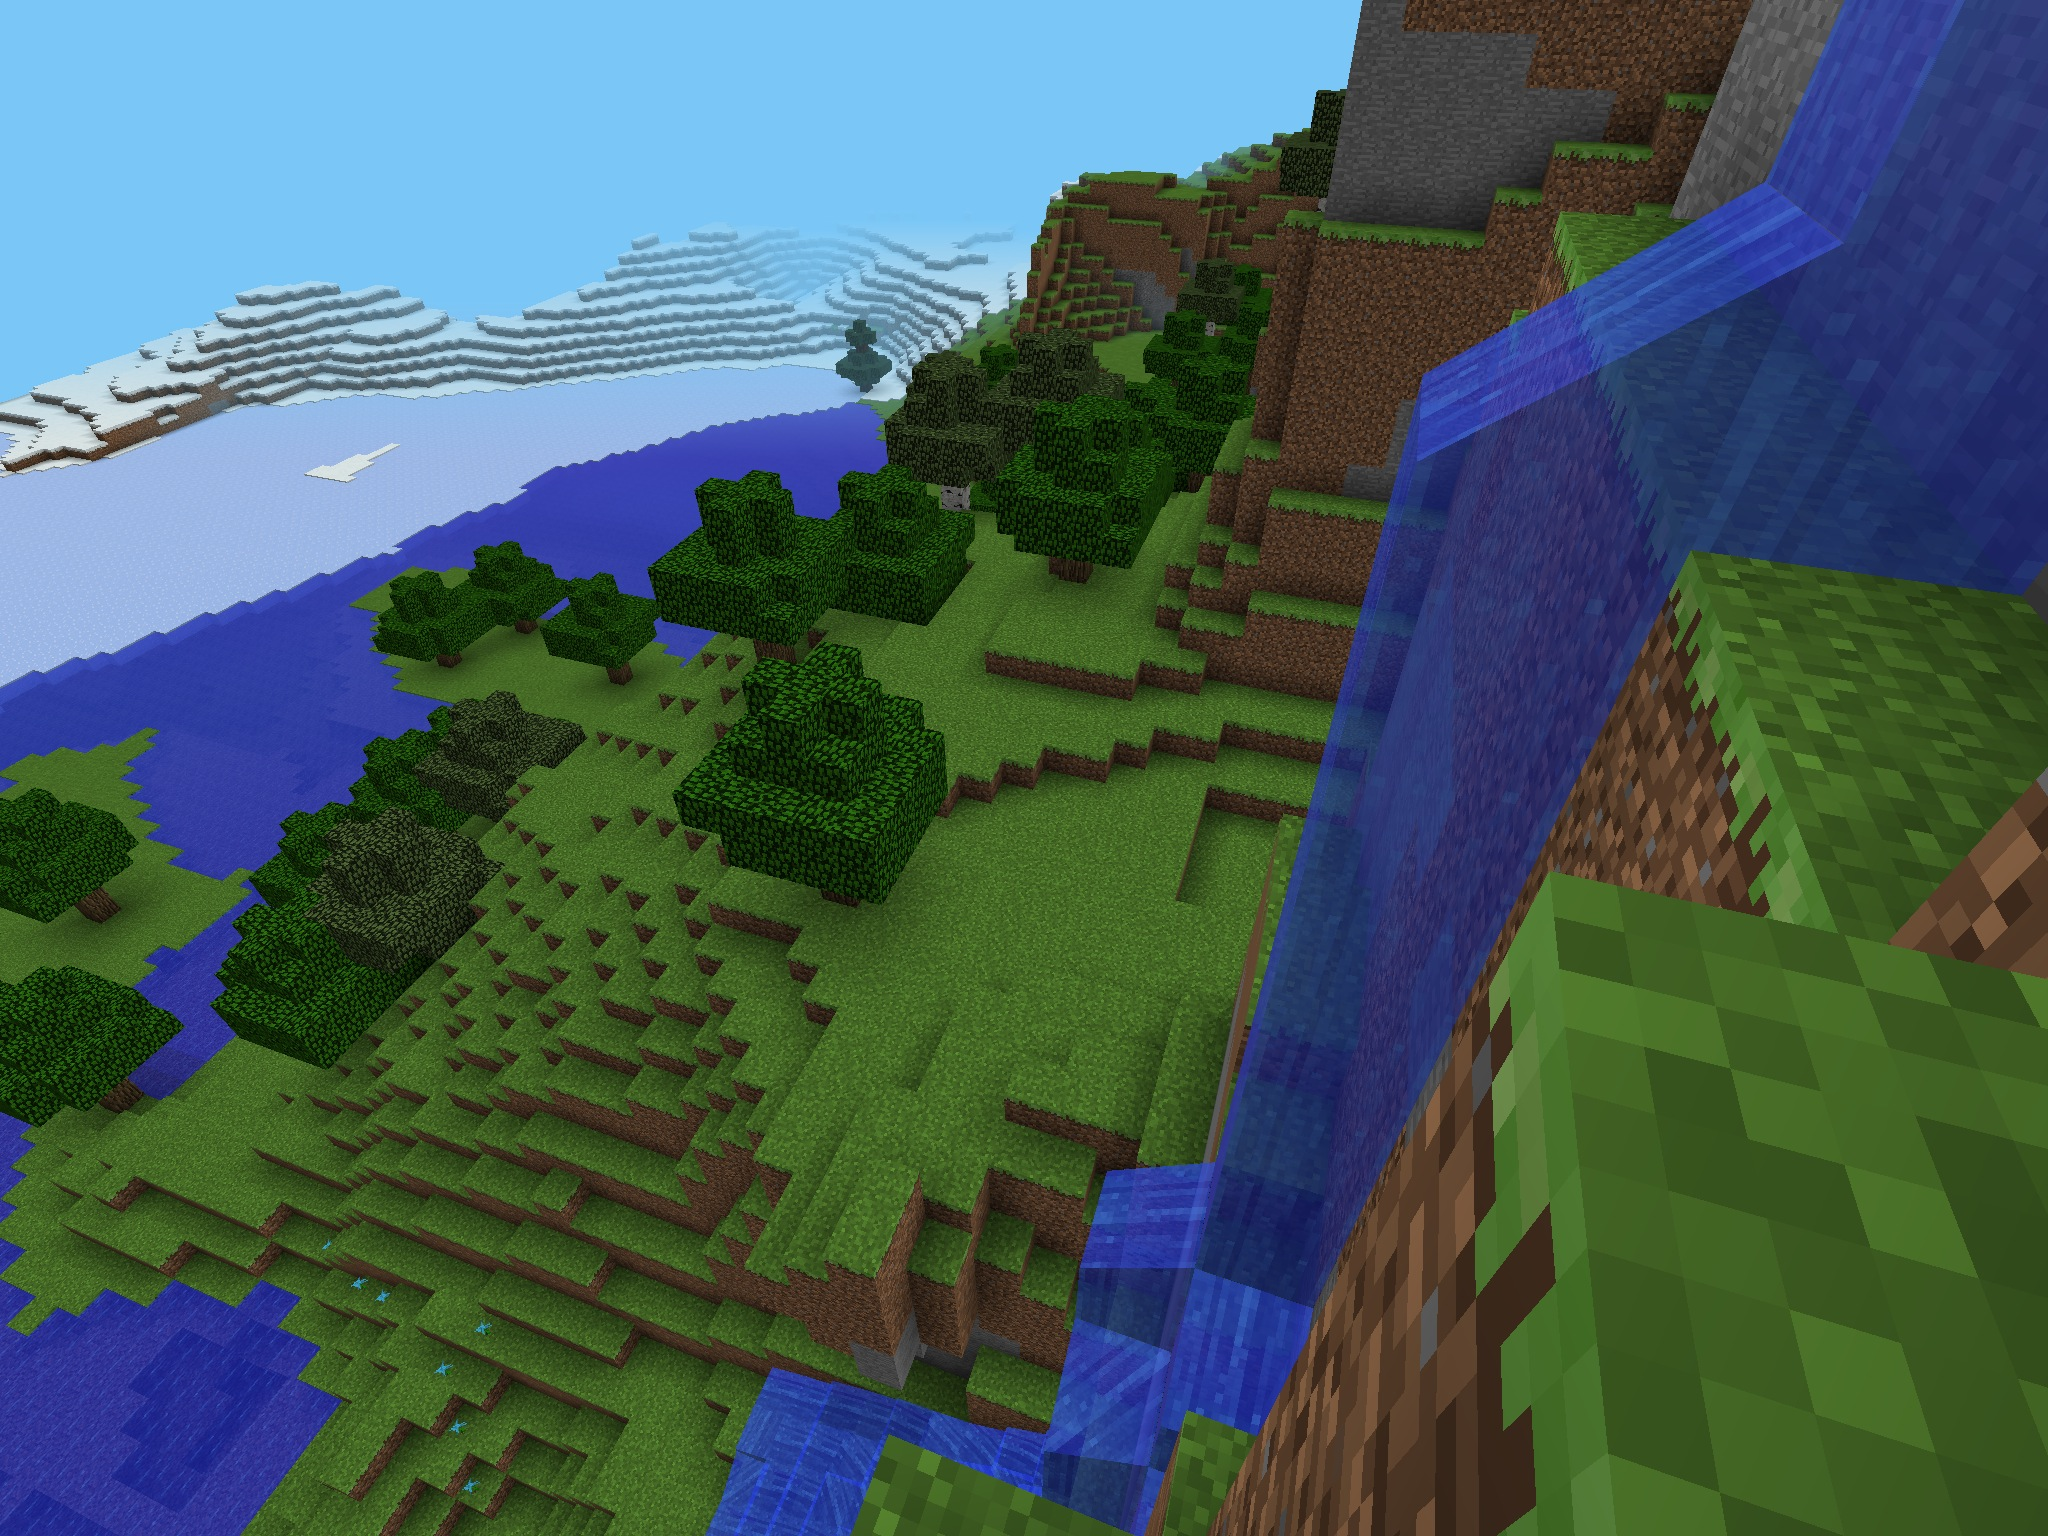
\includegraphics[width=0.5\linewidth]{obrazky-figures/miecraft.jpg}\hfill
	\caption{\textbf{Příklady celulárních simulací.} Na horním obrázku je simulace vytvořená během studia společně s~Bc. Petr Flajšingr. Na spodním obrázku je ukázána simulace vody ve známé hře Minecraft}
	\textbf{Zdroj: } \url{https://github.com/Nirvanios/Water_simulation-cellular_automaton} 
	\textbf{Zdroj: } \url{https://mcpedl.com/ayay/}
	\label{fig:SWE}
\end{figure*}

\section{Lagrangeova metoda toku}
Základem Lagrangeovy metody toku není sledování vymezeného prostoru, kde se může kapalina pohybovat, jako je tomu u~Eulerovy metody, ale sledovaní kapaliny samotné. Lagrangeova metoda se tak soustředí na celkovou kapalinu, kterou dělí na samostatné části. Lze tedy říci, že se jedná o~částicovou metodu, kde každá taková částice kapaliny nese specifické parametry jako hustotu, tlak, hmotnost a jiné. Pomocí těchto parametrů pak ovlivňuje ostatní částice v~okolí a tím i celou masu kapaliny.

Jak z~popisu vyplývá, tyto metody nejsou v~prostoru omezeny žádnou mřížkou, či jinou strukturou, limitující prostor dané simulace. Přestože nevzniká vysoká paměťová náročnost z~nutnosti mít mřížku, vyvstává paměťová náročnost v~podobě počtu částic. Pro dostatečně přesnou a jemnou simulaci, je totiž nutné mít vysoký počet částic. Počty částic se mohou pohybovat v~řádech od desítek tisíc až po jednotky či desítky miliónů. Při předpokladu  vysokého počtu částic a skutečnosti, že každá částice o~sobě musí nést mnoho informací jako je rychlost, pozice, hmotnost a další, je nutné počítat s~paměťovými nároky na jiném místě.

\subsection{Smoothed Particle Hydrodynamics}
\label{chapter:SPH}
Smoothed Particle Hydrodynamics (dále jen SPH) je dnes jednou z~nejpoužívanějších metod částicové simulace kapalin. Tato metoda byla představena autory Gingold a Monaghan \cite{Monaghan77} a Lucy \cite{Lucy77}, původně pro řešení problému v~teoretické astrofyzice. Postupem času se z~ní ale stala velice populární metoda, která se dočkala nespočtu rozšíření a modifikací a začala se používat nejen v~astrofyzice, ale také v~balistice, vulkanologii a především obecně v~oblastech simulace tekutin a jiných spojitých mas.

SPH je Lagrangeova metoda, základem jsou tedy částice. Každá částice nese několik konkrétních hodnot, jako je hmotnost, pozice a vektor rychlosti a navíc ještě několik dalších hodnot, vztahujících se k~danému problému, jako je hustota hmotnosti, tlak nebo například teplota. Jedná se o~integrační metodu, kde je výpočet konkrétního atributu $A(\mathbf{r})$ částice $I$ nad prostorem $\Omega$ definován pomocí rovnice \ref{eq:SPHint},
\begin{equation}
	A_I(\mathbf{r}) = \int_\Omega A(\mathbf{r}')W(\mathbf{r} - \mathbf{r'},h)\mathbf{dr}'
	\label{eq:SPHint}
\end{equation}
kde $r$ značí pozici v~prostoru, $W$ je vyhlazovací jádro (smoothing kernel) a $h$ je šířka jádra. Šířka jádra, nazývaná také vyhlazovací poloměr (smoothing radius) pak ovlivňuje kvalitu a stabilitu simulace. Z podmínek platících pro jádro popsaných níže, lze následně odvodit, že nová hodnota daného atributu je určitým průměrem hodnot okolních částic.
Numerický výpočet je pak zobrazen rovnicí \ref{eq:SPHsum},

\begin{equation}
	A_S(\mathbf{r}) = \sum_j A_j V_j W(\mathbf{r} - \mathbf{r_j},h)
	\label{eq:SPHsum}
\end{equation}

\begin{equation}
	V~= \frac{m}{\rho}
	\label{eq:volume}
\end{equation}
kde je integrál aproximovaný pomocí sumy přes všechny částice $j$ a $V$ je objem v~prostoru, který částice zaujímá přičemž je vypočítaný pomocí známé rovnice \ref{eq:volume}, kde $m$ je hmotnost částice a $\rho$ je hustota hmotnosti částice.  \cite{KelagerSPH}

\subsubsection{Vyhlazovací jádro}
Vyhlazovací jádro je jednou z~nejdůležitějších součástí celého SPH algoritmu a výběr správného jádra má tedy značný vliv na kvalitu a stabilitu simulace. Vhodné jádro musí splňovat dvě důležité podmínky.
\begin{equation}
	\int_\Omega W(\mathbf{r} - \mathbf{r}', h)\mathbf{dr}' = 1
	\label{eq:SPHCond1}
\end{equation}

\begin{equation}
	\lim{h \to 0} W(\mathbf{r} - \mathbf{r}',h) = \delta(\mathbf{r} - \mathbf{r}')
	\label{eq:SPHCond2}
\end{equation}

\begin{equation} \label{eq:dirac}
	\begin{gathered}
		\delta(x) =
		\begin{cases}
			\infty & \quad ||\mathbf{r}|| = 0 \\
			0      & \quad \text{jinak}
		\end{cases}
	\end{gathered}
\end{equation}
První podmínka \ref{eq:SPHCond1} udává, že jádro musí být normalizované, a nemůže tedy nikterak ovlivnit hodnoty, s~nimiž pracuje. Druhá podmínka \ref{eq:SPHCond2}, kde $\delta$ značí Diracovu delta funkci \ref{eq:dirac}, pak limituje počet interpolantů. Značí, že výsledek je ovlivněn pouze několika body v~okolí a body příliš vzdálené v~prostoru nikterak neovlivňují výsledek. V~původním článku autoři pro výpočet použili jedno-dimenzionální Gaussovské jádro (rovnice \ref{eq:1DGauss}). Jako další možnost je použít B-Splajn, kvintický splajn \cite{Liu2010} nebo například polynomiální kernel 6. stupně (rovnice \ref{eq:kernelPoly6}) \cite{Muller03}.

\begin{equation}
	W_{Gauss}(x,h) = \frac{1}{h\sqrt{\pi}}e^{-(x^2/h^2)}
	\label{eq:1DGauss}
\end{equation}

\begin{equation}
	W_{Poly6}(\mathbf{r},h) = \frac{315}{64 \pi h^9}
	\begin{cases}
		(h^2 - ||\mathbf{r}||^2)^3 & \quad 0 \leq ||\mathbf{r}|| \leq h \\
		0                          & \quad \text{jinak}
	\end{cases}
	\label{eq:kernelPoly6}
\end{equation}

\begin{figure}[hbt]
	\centering
	\captionsetup{justification=centering}
	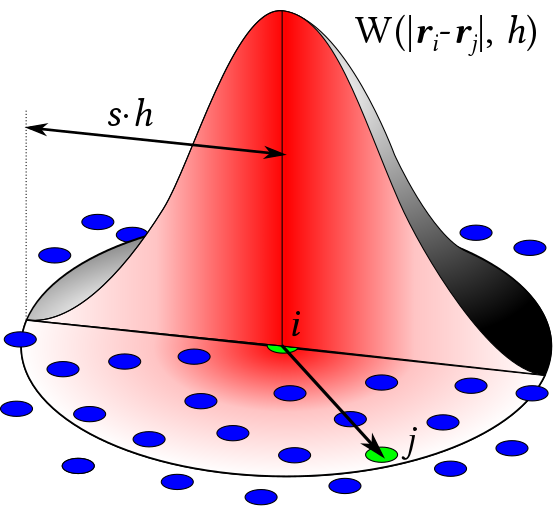
\includegraphics[width=0.4\textwidth]{obrazky-figures/SPHInterpolationColorsVerbose.png}
	\caption{\textbf{Vizualizace vyhlazovacího jádra.} Zelený bod $i$ je částice, pro kterou právě probíhá výpočet. Bod $j$ je pak jeden z bodů ovlivňující počítaný atribut částice $i$. Parametr $h$ následně udává poloměr jádra, který určuje oblast s částicemi přispívajícími k výpočtu. Samotné jádro je pak znázorněno trojrozměrnou Gaussovskou funkcí, která udává, jak velký význam daná částice má pro počítaný atribut. Vzdálenější částice nejsou tak významné v rámci výpočtu jako částice blíže k částici $i$}
	\textbf{Zdroj: } \url{https://en.wikipedia.org/wiki/Smoothed-particle_hydrodynamics}
	\label{fig:Kernel}
\end{figure}

\subsubsection{Hustota hmotnosti}
První veličinou, kterou je nutné vypočítat, je hustota hmotnosti pro každou konkrétní částici. Algoritmus SPH předpokládá, že hmotnost všech částic je během algoritmu neměnná a zároveň dopředu známá hodnota. Po kombinaci rovnic \ref{eq:SPHsum} a \ref{eq:volume} a dosazení hustoty $\rho$ jako počítaného atributu, vznikne následující rovnice \ref{eq:MassDensity} pro výpočet hustoty.


\begin{equation}
	\begin{split}
		\rho_i  & = \sum_i \rho_j V_j W(\mathbf{r_i} - \mathbf{r_j},h) \\
		& = \sum_i m_j W(\mathbf{r_i} - \mathbf{r_j},h)
	\end{split}
	\label{eq:MassDensity}
\end{equation}

\subsubsection{Tlak}
Tlak a síly působící díky tlaku jsou nesmírně důležité z~důvodu zachování nestlačitelnosti kapaliny. Dostane-li se větší shluk částic do jednoho místa, dojde k~lokálnímu zvýšení hustoty a tedy i tlaku a v~důsledku toho je nutné aplikovat takové síly, aby se shluk rozprostřel na větším prostoru. Tato síla je pak v~Navier-Stokesových rovnicích \ref{eq:NavierStokes} reprezentována termem $-\nabla p$. Pro výpočet tlakové síly působící na částici, lze opět aplikovat rovnici \ref{eq:SPHsum}, na ni známý vzorec \ref{eq:volume} a dosadit právě zmíněný term z~Navier-Stokesových rovnic.

\begin{equation}
	f^{tlak}_i = -\nabla p_i  & = \sum_i p_j \frac{m_j}{\rho_j} \nabla W(\mathbf{r_i} - \mathbf{r_j},h)
\end{equation}

Taková rovnice by však neprodukovala správné výsledky. Je-li uvažována simulace se dvěma částicemi, lze přijít na jeden zásadní problém, a to, že pomocí této rovnice není možné obdržet symetrické síly. Každá částice má lehce odlišný tlak, a proto tedy budou působící síly asymetrické. Existuje více způsobů jak symetrizovat tyto síly v~kontextu SPH. Nejjednodušším příkladem je následující rovnice \ref{eq:PressForce}. \cite{KelagerSPH} \cite{Monaghan92}

\begin{equation}
	f^{tlak}_i = -\sum_{i} \frac{p_i + p_j}{2} \frac{m_j}{\rho_j} \nabla W(\mathbf{r_i} - \mathbf{r_j},h)
	\label{eq:PressForce}
\end{equation}

Nyní, po získání symetrické tlakové síly, je poslední neznámou hodnota parametru $p$, označujícího tlak v~místě částice. Tuto hodnotu tlaku lze obdržet ze stavové rovnice ideálního plynu \ref{eq:idealGas},
\begin{equation}
	p = k\rho
	\label{eq:idealGas}
\end{equation}
kde $p$ je hledaný tlak, $k$ je plynová konstanta závislá na teplotě a $\rho$ je hustota vypočítaná pomocí rovnice \ref{eq:MassDensity}. Pro dosažení lepších výsledků lze také využít následující rovnice \ref{eq:idealGasRest},

\begin{equation}
	p_i = k(\rho_i - \rho_0)
	\label{eq:idealGasRest}
\end{equation}
kde $\rho_0$ označuje klidovou hustotu kapaliny. Jelikož síla závisí na gradientu pole tlaku, tento posun neovlivní výsledek sil, nicméně může učinit simulaci o~něco stabilnější.

Posledním problémem je výše popsané vyhlazovací jádro \ref{eq:kernelPoly6}. Zmíněné jádro má totiž snižovat velikosti odpuzujících sil, čím blíže částice jsou. Nastane-li tedy vysoký shluk částic, jádro není schopné produkovat dostatečné síly pro rovnoměrné rozprostření částic. Proto bylo navrženo \cite{Desbrun96} lepší jádro, schopné dané částice od sebe odtrhnout.

\begin{equation}
	W = (\mathbf{r}, h) = \frac{15}{\pi h^6}
	\begin{cases}
		(h - \mathbf{r})^3 & \quad 0 \leq ||\mathbf{r}|| \leq h \\
		0                  & \quad \text{jinak}
	\end{cases}
	\label{eq:pressureKernel}
\end{equation}

\subsubsection{Viskozita}
Při aplikaci dosavadních rovnic a postoupení k~integraci (viz. níže), je výsledkem simulace neviskózní kapaliny. V~reálném světě má však za běžných podmínek každá kapalina určitou viskozitu. Viskozitu lze chápat jako působení sil bránící kapalině ve změně tvaru z~důvodu vnitřního tření. Pro zavedení rovnice na výpočet síly působící díky viskozitě jsou použity opět Navier-Stokesovy rovnice, tentokrát term pro viskozitu $\mu \nabla^2\mathbf{u}(\mathbf{r_i})$ a opět obecnou rovnici pro SPH \ref{eq:SPHsum} společně s rovnici pro objem \ref{eq:volume}.

\begin{equation}
	f^{viskozita}_i = \mu \nabla^2\mathbf{u}(\mathbf{r_i}) = \mu \sum_i \mathbf{u_j} \frac{m_j}{\rho_j} \nabla^2 W(\mathbf{r_i} - \mathbf{r_j},h)
\end{equation}

Zde nastává stejný problém, jako u~tlakových sil, a to že jsou síly opět asymetrické. Správného výsledku pak můžeme dosáhnout následující rovnicí \ref{eq:ViscForce}. \cite{Muller03}

\begin{equation}
	f^{viskozita}_i = \mu \sum_i m_j \frac{\mathbf{u_i} - \mathbf{u_j}}{\rho_j} \nabla^2 W(\mathbf{r_i} - \mathbf{r_j},h)
	\label{eq:ViscForce}
\end{equation}

Viskozita je vlastnost tekutiny, která do celého systému ze svého principu nepřináší energii, a tedy v~celé tekutině nikterak nevzrůstá rychlost. Avšak jak polynomiální jádro šestého řádu \ref{eq:kernelPoly6}, tak jádro použité pro výpočet tlaku \ref{eq:pressureKernel}, může do systému takové zvýšení energie zanést. Je nutné tedy najít takové jádro, které pouze snižuje velikost sil v~závislosti na velikosti viskozity. Následující jádro \ref{eq:viscKernel} tuto podmínku splňuje. \cite{Muller03}

\begin{equation}
	W = (\mathbf{r}, h) = \frac{15}{2 \pi h^3}
	\begin{cases}
		-\frac{||\mathbf{r}||^3}{2h^3} + \frac{||\mathbf{r}||^2}{h^2} + \frac{h}{2||\mathbf{r}||} & \quad 0 \leq ||\mathbf{r}|| \leq h \\
		0                                                                                         & \quad \text{jinak}
	\end{cases}
	\label{eq:viscKernel}
\end{equation}

\begin{figure}[hbt]
	\centering
	\captionsetup{justification=centering}
	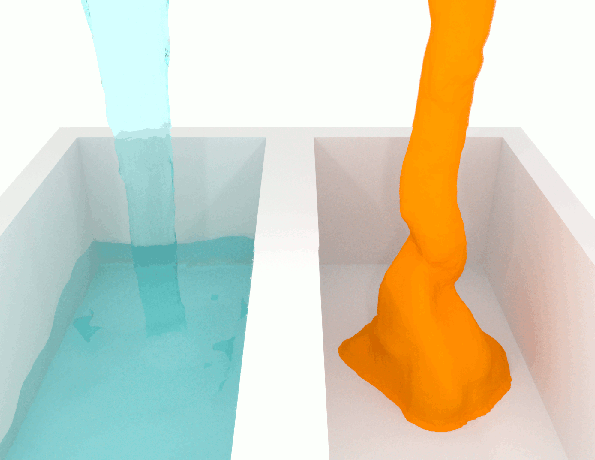
\includegraphics[width=0.5\textwidth]{obrazky-figures/viskozita.PNG}
	\caption{\textbf{Viskozita kapalin.} Případy různé viskozity, kapalina vpravo představující viskóznější kapalinu se mnohem více brání toku než méně viskózní kapalina vlevo.}
	\textbf{Zdroj: } \url{https://en.wikipedia.org/wiki/Fluid_animation}
	\label{fig:Vics}
\end{figure}

\subsubsection{Povrchové napětí}
Povrchové napětí je síla působící na vnější povrch kapaliny, přesněji řečeno se jedná o~nerovnováhu sil. Každá molekula kapaliny vytváří síly přitahující ostatní molekuly v~kapalině, jež jsou poblíž. Uvnitř kapaliny jsou síly vyrovnané, ale jak znázorňuje obr. \ref{fig:SurTen}, molekuly na okraji kapaliny jsou pouze přitahovány do pomyslného středu kapaliny. Povrchové napětí sice není přítomno v~Navier-Stokesových rovnicích, nicméně se jedná o~velice důležitou součást chování kapalin. Povrchové napětí totiž zapříčiňuje minimalizaci povrchu kapaliny, kterou lze v~přírodě pozorovat. \cite{KelagerSPH}

\begin{figure}[hbt]
	\centering
	\captionsetup{justification=centering}
	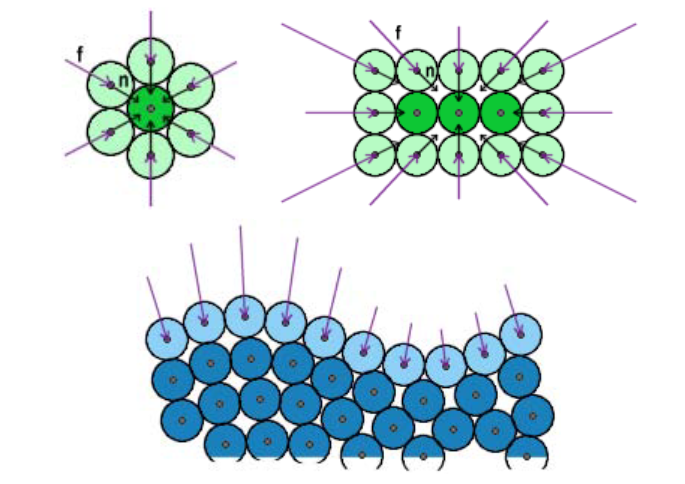
\includegraphics[width=0.7\textwidth]{obrazky-figures/SurfTens.png}
	\caption{\textbf{Povrchové napětí.} Různé případy povrchového napětí. U zelené kapaliny jsou částice k sobě přitahovány tak, že jsou síly navzájem vyrušeny. U modré kapaliny jsou Světle modré částice přitahovány k tmavě modrým a dochází tak působení sil, které vyvolává vlastnost zachování si nejmenšího povrchu kapaliny.}
	\textbf{Zdroj: } Lagrangian Fluid Dynamics Using Smoothed Particle Hydrodynamics \cite{KelagerSPH}
	\label{fig:SurTen}
\end{figure}

\begin{equation}
	f_i^{\text{\textit{povrchové napětí}}} = \sigma \nabla^2 c_i \frac{\mathbf{n}_i}{||\mathbf{n}_i||}
	\label{eq:SurfTen}
\end{equation}

Pomocí výše zmíněné rovnice \ref{fig:SurTen} pak lze vypočítat sílu povrchového napětí. V~rovnici $\sigma$ představuje koeficient povrchového napětí, specifický pro danou kapalinu, $c$ je tzv. barevné pole a $\mathbf{n}$ je normála povrchu kapaliny směřující dovnitř. Barevné pole $c$ je definováno podmínkou \ref{eq:color}.

\begin{equation}
	c_i =
	\begin{cases}
		1 & \quad  \text{na pozici částice } i \\
		0 & \quad  \text{jinde}
	\end{cases}
	\label{eq:color}
\end{equation}
S~pomocí rovnice \ref{eq:SPHsum} lze pak pole $c_i$ vypočítat následující rovnicí \ref{eq:ColorField}.

\begin{equation}
	\begin{split}
		c_i =   & \sum_j c_j V_j \nabla^2 W(\mathbf{r_i} - \mathbf{r_j},h) \\
		=   & \sum_j V_j \nabla^2 W(\mathbf{r_i} - \mathbf{r_j},h)
	\end{split}
	\label{eq:ColorField}
\end{equation}

Z~gradientu barevného pole pak lze získat normálu povrchu $\mathbf{n}_i$.
\begin{equation}
	\mathbf{n}_i = \nabla c_i
	\label{eq:SurfNormal}
\end{equation}

Podmínka vyhodnocení je omezena členem $\frac{\mathbf{n}_i}{||\mathbf{n}_i||}$, kde $||\mathbf{n}_i||$ nabývá nenulových hodnot pouze blízko okraje kapaliny. Pokud je však $||\mathbf{n}_i||$ příliš malé, způsobuje numerickou nestabilitu řešení, a proto se síla povrchového napětí počítá jen v~případě, kdy $||\mathbf{n}_i||$ překročí jistý práh.


\subsubsection{Síly}
Síly působící na kapalinu lze rozdělit do dvou kategorií, vnitřní a vnější síly. Pro výpočet celkové síly působící na jednu částici v~systému pak stačí vnější a vnitřní síly sečíst. Vnitřní a vnější síly jsou definovány rovnicemi \ref{eq:ForceInt} a \ref{eq:ForceExt} následovně, \cite{KelagerSPH}

\begin{equation}
	f^{\text{\textit{vnitřní}}} = f^{tlak} + f^{viskozita}
	\label{eq:ForceInt}
\end{equation}

\begin{equation}
	f^{\text{\textit{vnější}}} = f^{\text{\textit{povrchové napětí}}} + f^{gravitace}
	\label{eq:ForceExt}
\end{equation}
kde je síla působící z~důvodu gravitace vyjádřena rovnicí \ref{eq:forceGrav}, přičemž $g$ značí gravitační zrychlení.

\begin{equation}
	f^{gravitace} = \rho g
	\label{eq:forceGrav}
\end{equation}
Posledním důležitým krokem je výpočet zrychlení částice \ref{eq:Acc} z~důvodu působení sil.

\begin{equation}
	a_i = \frac{f^{vnejsi} + f^{vnitri}}{\rho}
	\label{eq:Acc}
\end{equation}

\subsubsection{Integrace}
Nyní představené vzorce jsou vše potřebné pro základní SPH simulaci, nicméně pouhým výpočtem výše popsaných vlastností hodnot nelze dostat tekoucí kapalinu. Je nutné každou částici vždy posunout v~čase a prostoru na základě předchozí pozice, rychlosti a působících sil. Existuje několik přístupů jak numericky řešit posun částic v~čase a prostoru.

Mezi nejznámější a nejjednodušší metodu numerické integrace patří Eulerova metoda. V~její nejjednodušší formě se pozice i rychlost (rovnice \ref{eq:eulerU} a \ref{eq:eulerR}) aktualizují zároveň na základě vypočtených hodnot.

\begin{equation}
	\mathbf{u}_{t + \Delta t} = \mathbf{u}_t + \Delta t \mathbf{a}_t
	\label{eq:eulerU}
\end{equation}

\begin{equation}
	\mathbf{r}_{t + \Delta t} = \mathbf{r}_t + \Delta t \mathbf{u}_t
	\label{eq:eulerR}
\end{equation}

Existuje lehké zlepšení metody, ve kterém se následující pozice počítá z~již vypočítané rychlosti. Výpočet pozice tedy závisí na výpočtu rychlosti. Ve výpočtu je následně rovnice \ref{eq:eulerR} nahrazena rovnicí \ref{eq:eulerR2}. \cite{KelagerSPH}

\begin{equation}
	\mathbf{r}_{t + \Delta t} = \mathbf{r}_t + \Delta t \mathbf{u}_{t + \Delta t}
	\label{eq:eulerR2}
\end{equation}

Dalším vylepšením může být integrační metoda Leap-Frog. Tato metoda vychází z~Eulerovy metody, nicméně zavádí posunutí výpočtu rychlosti v~čase. Výpočet rychlosti je posunut o~$\frac{\Delta t}{2}$, čímž dochází ke \enquote{střídání} výpočtu rychlosti a pozice, viz. obr. \ref{fig:LeapFrog}. Vzorce pro výpočet rychlosti \ref{eq:LeapVel} a pozice \ref{eq:LeapPos} jsou následující.

\begin{equation}
	\mathbf{u}_{t + \frac{\Delta t}{2}} = \mathbf{u}_{t - \frac{\Delta t}{2}} t \mathbf{a}_t
	\label{eq:LeapVel}
\end{equation}

\begin{equation}
	\mathbf{r}_{t + \Delta t} = \mathbf{r}_t + \Delta t \mathbf{u}_{t + \frac{\Delta t}{2}}
	\label{eq:LeapPos}
\end{equation}

\begin{figure}[hbt]
	\centering
	\captionsetup{justification=centering}
	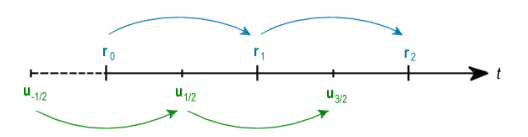
\includegraphics[width=0.7\textwidth]{obrazky-figures/leapFrog.PNG}
	\caption{\textbf{Leap-Frog integrace.} Vyobrazení posunutí integrace rychlosti a pozice mezi sebou. Pozice $r$ je počítána v čase $t$, zároveň s ní je počítána rychlost $u$ pro čas $t+\frac{1}{2}$ vycházející z rychlosti $u$ v čase $t-\frac{1}{2}$}
	\textbf{Zdroj: } Lagrangian Fluid Dynamics Using Smoothed Particle Hydrodynamics \cite{KelagerSPH}
	\label{fig:LeapFrog}
\end{figure}

\newpage

\subsubsection{Algoritmus simulace}

\begin{center}
	\begin{czechalgorithm}[H] \label{alg:SPH}
			\ForEach{\text{particle}} {\\
				vypočti hustotu (viz. \ref{eq:MassDensity})\\
				vypočti tlak (viz. \ref{eq:idealGasRest})\\
			}\\
			\\
			\ForEach{\text{particle}} {\\
				vypočti tlakovou sílu $f^{tlak}_i$ (viz. \ref{eq:PressForce})\\
				vypočti viskózní sílu $f^{viskozita}_i$ (viz. \ref{eq:ViscForce})\\
				vypočti vlastní hodnotu barevného pole $c_i$ (viz. \ref{eq:ColorField})\\
				vypočti normálu povrchu kapaliny $\mathbf{n}_i$ (viz. \ref{eq:SurfNormal})\\
				vypočti sílu povrchového napětí $f^{\text{povrchové napětí}}_i$ (viz. \ref{eq:SurfTen})\\
				$f^{vnitrni} = f^{tlak}_i f^{viskozita}_i$ \\
				$f^{vnitrni} = f^{\text{povrchové napětí}}_i + f^{gravitace}_i$\\
				$f = f^{vnejsi} + f^{vnitrni}$ (viz. \ref{eq:ForceExt} a \ref{eq:ForceInt})\\
				vypočti zrychlení $a_i$ (viz. \ref{eq:Acc})\\
				integruj a posuň částici v~čase (viz. \ref{eq:LeapPos} a (viz. \ref{eq:LeapPos})\\
			}\\

		\caption{Krok SPH Simulace}
	\end{czechalgorithm}
\end{center}

\begin{figure*}[h]\centering
	\centering
	\captionsetup{justification=centering}
	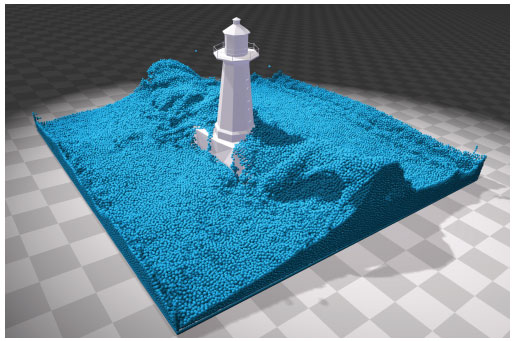
\includegraphics[width=0.5\linewidth]{obrazky-figures/SPHSim1_01.jpg}\hfill
	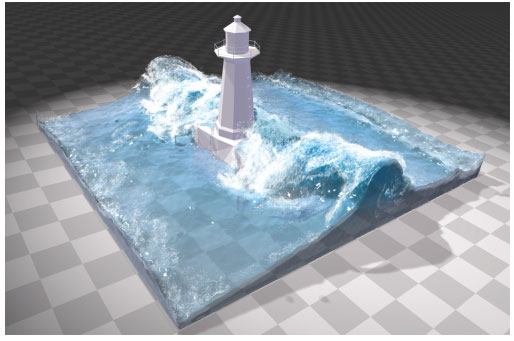
\includegraphics[width=0.5\linewidth]{obrazky-figures/SPHSim1_02.jpg}\hfill
	\caption{\textbf{Příklady SPH Simulace.} Na levém obrázku je simulace zobrazená pomocí jednotlivých částic. Na pravém obrázku je ukázána vyrenderovaná hladina}
	\textbf{Zdroj: } SPH Fluids in Computer Graphics \cite{Ihmsen14}
	\label{fig:SPHFigure}
\end{figure*}

\chapter{Návrh řešení}
\label{chapter:navrh_resení}
Důležitou součástí celého procesu tvorby simulátoru je vytvořit si návrh celého systému. Je důležité zvolit vhodný jazyk pro implementaci, vhodné grafické/výpočetní API, ale také celkovou podobu programu, jeho vzhled, funkčnost a v neposlední řadě rozhraní mezi uživatelem a samotným programem. V následujících podkapitolách jsou tak tyto problémy probrány a zdůvodněny výběry daných řešení. 

\section{Specifikace požadavků}
\label{chapter:spec}
Implementace výše uvedených algoritmů v sekci \ref{chapter:Grid} a \ref{chapter:SPH} již existuje a to od projektů implementuijící základy jako je například SPH 3D Real-Time Fluid Simulation \footnote{\url{https://github.com/saeedmahani/SPH-3D-Fluid-Simulation}}, přes složitější projekty implementující několik různých přístupů k simulaci napříkald C++ Fluid Particles \footnote{\url{https://github.com/TroyZhai/CPP-Fluid-Particles}} až po komplexní řešení ve formě knihoven jako je SPHysics \footnote{\url{https://wiki.manchester.ac.uk/sphysics/index.php/Main_Page}} či SPlisHSPlasH~\footnote{\url{https://github.com/InteractiveComputerGraphics/SPlisHSPlasH}}. Při běžném hledání na internetu lez dokonce najít implementace běžící ve webovém prohlížeči s použitím javascriptového WebGL API. Mezi zmínky patří například WebGL Fluid Simulation \footnote{\url{https://github.com/PavelDoGreat/WebGL-Fluid-Simulation}} či Fluid Particles \footnote{\url{https://github.com/dli/fluid}}. Z důvodu existence celé řady implementací a to jak Eulerovy mřížkové metody tak algoritmu Smoothed Particle Hydrodynamics, bylo nutné vybrat přístup k simulaci, případně jev, který není tak hojně představován. Z tohoto důvodu byl vybrán článek autorů Hochstetter a Kolb popisující vypařování a kondenzaci kapalin. Z důvodu komplexnosti celého tématu, byl však vybrán pouze jeden jev a to vypařování kapalin.

Hlavním požadavkem výsledné aplikace je schopnost odsimulovat tekutinu nacházející se v nějakém předem definovaném prostoru, vizualizovat současný stav kapaliny ve formě částic či objemu a možnost celý průběh simulace řídit. Uživatel má tedy přístup k ovládacím prvkům schopných simulaci pozastavit, krokovat či resetovat do výchozího stavu. Pro testování v rámci implementace, ale následně i používání aplikace se jeví jako vhodné využít také ukládání současného stavu simulace a jeho případné opětovné načtení. dalším požadavkem je možnost aplikace reprodukovat výslednou simulaci a to z důvodů především prezentačních, ale i z důvodu rychlosti výpočtu simulace. Simulace jako takové jsou často velmi náročné na výpočet a pro stabilní simulaci je třeba zvolit nízký krok simulace, což v kombinaci s náročnými výpočty může vést k výpočtu řádově jednotek snímků za vteřinu, případně několik vteřin či minut na snímek v případně složitějších simulací. Z toho důvodu je vhodné aby aplikace mohla celý průběh simulace nahrávat a následně celý proces simulace zobrazit v reálném čase. 

Jak bylo však již zmíněno v úvodu, tato práce je zaměřená především na prozkoumání možností v oblasti simulace kapalin, načerpání nových informací a rozšíření okruhu znalostí. Z toho důvodu hlavním cílem této práce není přinést revoluční model simulace kapalin, přidat nějaký dříve opomíjený jev související s chováním kapalin, či snad poukázat na chyby v jiných modelech. Tato práce si tedy klade za cíl proniknout do poměrně zajímavého okruhu simulace tekutin, implementovat a předvést její základy, ale také se také zlepšit jak v běžném programování, tak v práci s grafickými výpočetními jednotkami a jejich využití, při provádění paralelních výpočtů. Výsledná aplikace tak nemá ambice býti \enquote{state-of-the-art} produktem v oblasti výpočtů dynamiky kapalin, nicméně se spíše jedná o prezentaci nastudovaných materiálů a jejich aplikace v praxi.

\begin{figure*}[h]\centering
	\centering
	\captionsetup{justification=centering}
	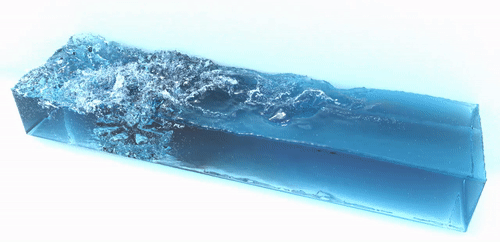
\includegraphics[width=0.5\linewidth]{obrazky-figures/splish-0.png}\hfill
	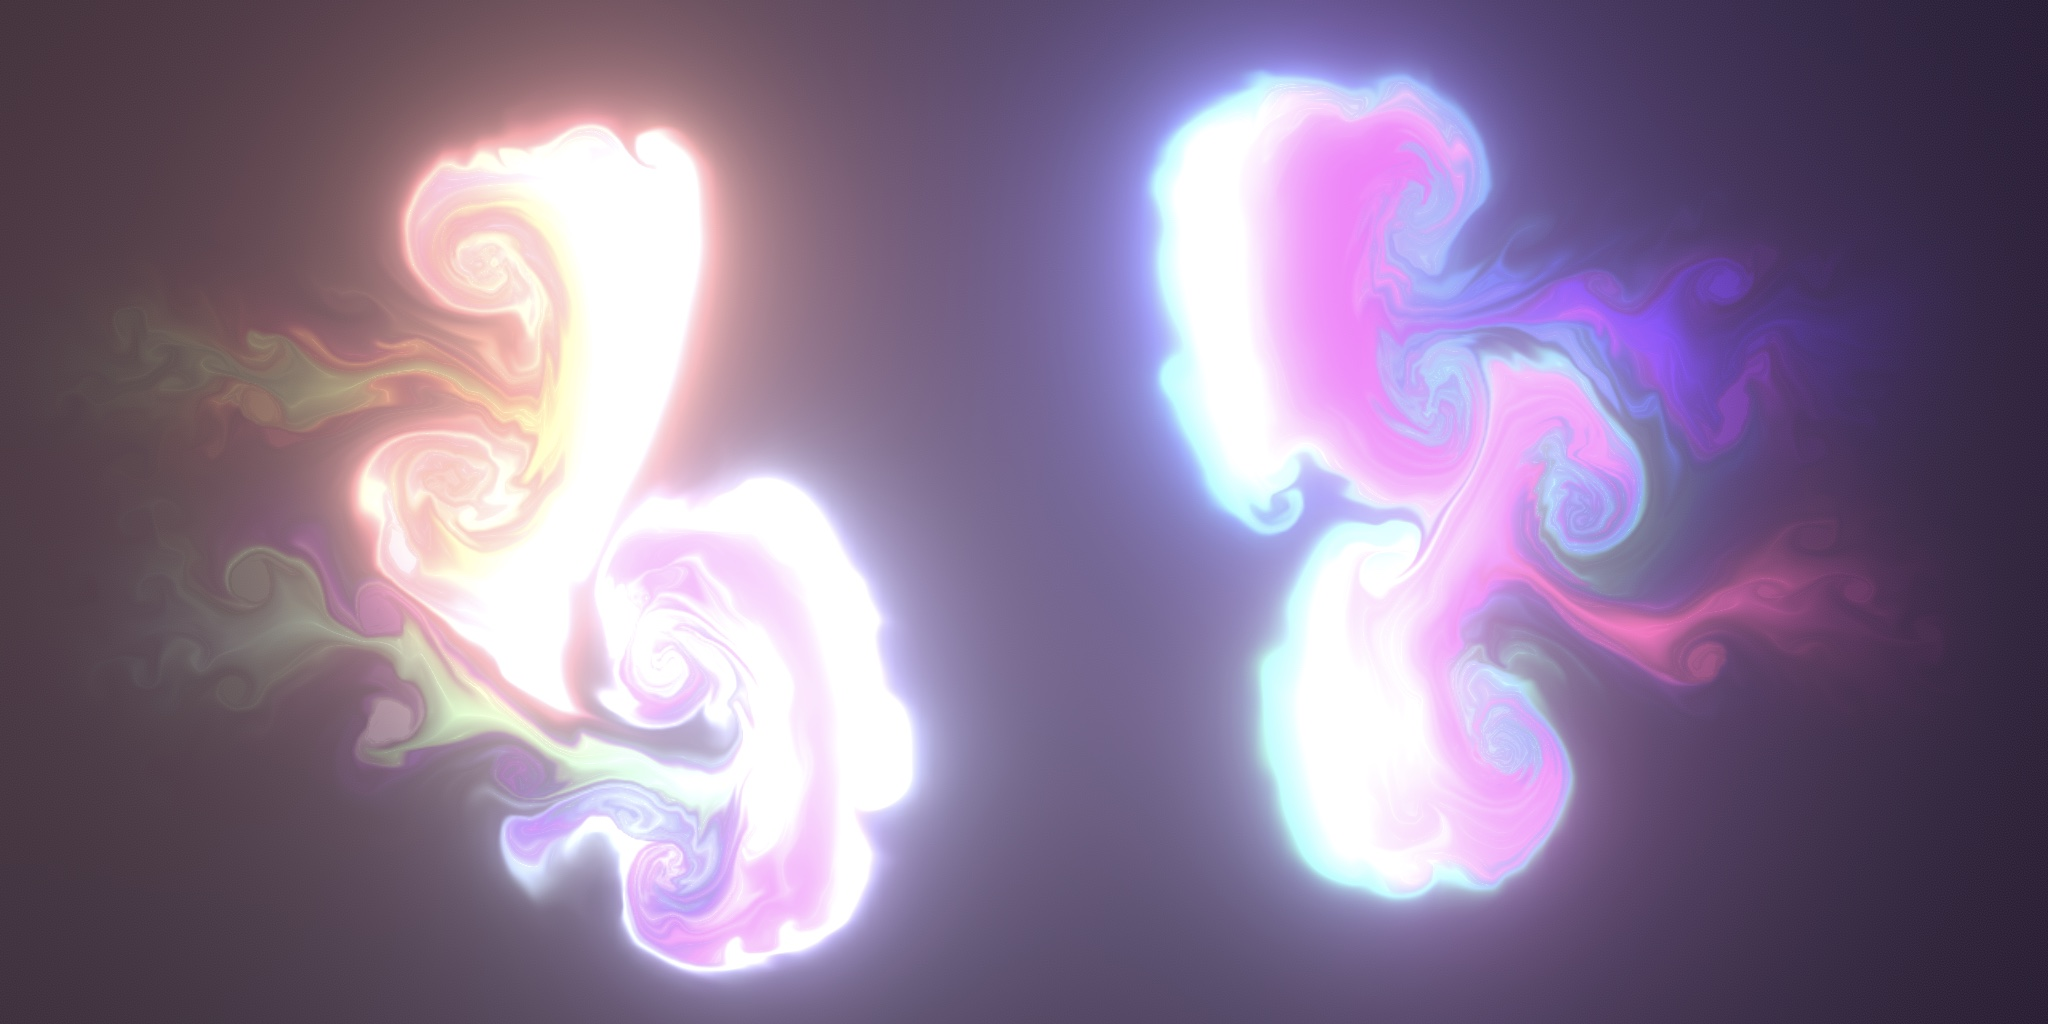
\includegraphics[width=0.5\linewidth]{obrazky-figures/webglFluid.jpg}\hfill
	\caption{\textbf{Existující řešení.} Na obrázku vlevo je znázorněna částicová simulace z knihovny SPlisHSPlasH. V pravo pak lze videt výsledek z Eulerovy mřížkové metody z webové aplikace WebGL Fluid Simulation }
	\textbf{Zdroj: } \url{https://github.com/InteractiveComputerGraphics/SPlisHSPlasH} \newline
    \textbf{Zdroj: } \url{https://github.com/PavelDoGreat/WebGL-Fluid-Simulation}
	\label{fig:existingSolution}
\end{figure*}

\section{Propojení simulací}
\label{chapter:evap}
Tato práce se tedy zaměřuje mimo jiné na článek \cite{Evap&Cond} autorů Hochstetter a Kolb z~University of Siegen v~Německu, který se snaží implementovat. Ačkoliv se s~kondenzací a vypařováním lze setkat běžně každý den, v~rámci simulace kapalin a počítačové grafiky není mnoho prací věnujících se tomuto tématu. Z~tohoto důvodu se pomocí zmíněného článku snaží autoři představit novou metodu, jak takové změny skupenství simulovat. Autoři se rozhodli využít dvou metod simulace. Pro kapalné skupenství využili metodu Smoothed Particle Hydrodynamics (viz. kapitola \ref{chapter:SPH}), plynné skupenství pak bylo simulováno za využití mřížkové metody (viz. kapitola \ref{chapter:Grid}). Pro kondenzaci na povrchu pevných těles následně využili textur nesoucích potřebné údaje. Přestože se tato práce zabývá implementací pouze vypařování kapalin, je zde podrobněji celá metoda popsána a to včetně kondenzace, celý popis pak vychází z~článku napsaného autory. \cite{Evap&Cond}

\subsubsection{Základní princip}
Popisovaná simulace se skládá ze tří částí, částicový systém pro simulaci kapalného stavu, mřížkový systém pro simulaci plynného stavu a textury udržující informace o~množství kondenzace na pevných tělesech. Principy SPH simulace a mřížkové metody již byly popsány výše v~kapitolách \ref{chapter:SPH} a \ref{chapter:Grid} respektive, avšak pro správné fungování cyklu vypařování a kondenzace je nutné do obou systémů zavést novou veličinu, a to teplotu.

u mřížkové metody se nejedná o žádný velký zásah. Jedná o~pouhé advekování teploty a hustoty pomocí pole vektorů rychlostí. Postup veličin polem je popsán následujícími rovnicemi \ref{eq:advTemp} a \ref{eq:advRho}.
\begin{equation}
	\frac{\partial T}{\partial t} = -(\mathbf{u} \cdot \nabla)T
	\label{eq:advTemp}
\end{equation}

\begin{equation}
	\frac{\partial \rho}{\partial t} = -(\mathbf{u} \cdot \nabla)\rho
	\label{eq:advRho}
\end{equation}

Pro zachování vlastnosti plynů, kdy horký plyn stoupá a těžký studený plyn klesá, je nutné zavést do systému vztlakovou sílu. Ta je popsána následující rovnicí \ref{eq:buoyEvap} a je součástí parametru $f$ rovnice \ref{eq:NavierStokes},

\begin{equation}
\label{eq:buoyEvap}
	f_{buoy} = -\alpha \rho \hat{\mathbf{g}} + \beta(T - T_{amb})\hat{\mathbf{g}}
\end{equation}
kde $\alpha$ a $\beta$ jsou předem definované konstanty a $\hat{\mathbf{g}}$ je normalizovaný vektor gravitačního zrychlení.

Pro SPH simulaci je nutné počítat pro každou částici také teplotu. Pro modelování teploty v~rámci kapaliny využili autoři článku rovnici \ref{eq:SPHTemp} vytvořenou dvojící Cleary a Monaghan \cite{Cleary99}, 

\begin{equation}
	\frac{\partial T}{\partial t} = \frac{V_1}{m_i C_i} \sum_j \frac{4 k_i k_j}{k_i + k_j} V_j \frac{(T_i - T_j)}{||\mathbf{r}_i - \mathbf{r}_j||}\nabla W(\mathbf{r} - \mathbf{r_j},h)
	\label{eq:SPHTemp}
\end{equation}
přičemž $C_i$ označuje tepelnou kapacitu částice $i$ a $k_i$ tepelnou vodivost.

Nakonec jsou vytvořeny textury pro pevné tělesa. Každému tělesu náleží několik textur. Základní textura v~každém texelu obsahuje množství zkondenzované kapaliny. Použitím textury a texelů menší než je částice z~SPH simulace je docíleno jemnějšího detailu při kondenzaci. Dále je k dispozici přepočítaná textura obsahující hodnotu maximálního množství kapaliny v~daném texelu a texturu obsahující mapu pozic pro vytváření SPH částic. Další textury obsahují například teplotu, případně historii kondenzace.

\subsubsection{Míra kondenzace a vypařování}
Při vypařování a kondenzaci je nutné zjistit množství hmoty, které se transformuje z~jednoho skupenství do druhého, pro výpočet změny hmotnosti v~povrchu kapaliny je nabízen následující vzorec \ref{eq:EvapRate} založený na empirických datech. \cite{SMITH94}

\begin{equation}
	\frac{\partial m_s}{\partial t} = A_s(a + b \cdot ||\mathbf{u}||)(p_s^{sat} - p_c)
	\label{eq:EvapRate}
\end{equation}

Kde $A_s$ je plocha kontaktu kapaliny, $a$ a $b$ jsou konstanty ovlivňující vypařování a $p_s^{sat}$ je tlak nasycených výparů u~povrchu kapaliny a $p_c$ je tlak výparu v~buňce. Hodnoty tlaků jsou vypočítány následujícími rovnicemi \ref{eq:evapPress} a \ref{eq:evapSatur}. \cite{yau1996short}

\begin{equation}
	p_c = \frac{m_c R_w(T_c - 273,15^{\circ}C)}{V_c}
	\label{eq:evapPress}
\end{equation}

\begin{equation}
	p_s^{sat} = 611.2\text{Pa} e^{\frac{17,62 \cdot T_s}{243,12^{\circ}C + T_s}}
	\label{eq:evapSatur}
\end{equation}

Z rovnice \ref{eq:EvapRate} je získána míra vypařování z~povrchu kapaliny, nicméně míru kondenzace lze vyjádřit s~pomocí stejné rovnice. V~závislosti na znaménku výsledku dané rovnice lze následně určit, zda se jedná o~kondenzaci či vypařování. Z toho vyplývají následující rovnice \ref{eq:EvapTrans} a \ref{eq:CondTrans},

\begin{equation}
	\textit{míra vypařování}(c,s) = \max\left(\frac{\partial m_s}{\partial t}, 0\right)
	\label{eq:EvapTrans}
\end{equation}

\begin{equation}
	\textit{míra kondenzace}(c,s) = \min\left(\frac{\partial m_s}{\partial t}, 0\right), \text{kde } b = 0
	\label{eq:CondTrans}
\end{equation}
přičemž $c$ značí buňku a $s$ značí surfel, tedy povrchovou jednotku kapaliny. Pro zjištění hodnot buňky na konkrétní pozici $\mathbf{r}$ lze využít například trilineární interpolace hodnot buněk v~okolí. Rovnice \ref{eq:EvapRate} přináší určitou závislost vypařování na proudění vzduchu v~okolí, nicméně kondenzace v~žádném případě nezávisí na okolní rychlosti vzduchu, proto jej lze z~rovnice vyškrtnout za pomocí argumentu $b=0$. Nakonec je nutné při každém přenosu zajistit, aby se z~kapaliny odebralo stejné množství hmotnosti, jako je přijato do plynné fáze. Je tedy usilováno o zajištění zákonu o~zachování hmotnosti a nezpůsobovat úbytek či přírůstek hmotnosti v~celém systému simulace.

\subsubsection{Simulace}
Pro správné fungování simulace, přenosů tepla a hmotností je nutné veškeré systémy propojit. Je zapotřebí přenos teplot mezi kapalinou a výpary a texturami a částicemi. Pevná tělesa jsou reprezentována pomocí částic, a to z~důvodu snadnější interakce kapalina~$\leftrightarrow$~\mbox{těleso} nejen v~rámci sil, ale i přenosu tepla. Zároveň musí docházet k~přenosu hmotnosti mezi všemi třemi systémy. Celé propojení je znázorněné na obrázku \ref{fig:EvapCycle}.

\begin{figure}[hbt]
	\centering
	\captionsetup{justification=centering}
	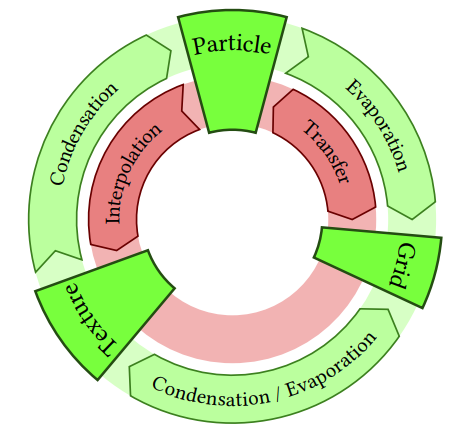
\includegraphics[width=0.4\textwidth]{obrazky-figures/evapCycle.PNG}
	\caption{\textbf{Propojení tří systémů.} Zelený kruh zobrazuje přenos hmotnosti a červený kruh přenos teploty.}
	\textbf{Zdroj: } Evaporation and condensation of SPH-based fluids \cite{Evap&Cond}
	\label{fig:EvapCycle}
\end{figure}

\subsubsection{Přenos tepla}
Pro fungování simulace je nutné vytvořit přenos tepla částice $\leftrightarrow$ buňka a jelikož se pevná tělesa sestávají z~částic tak také částice $\leftrightarrow$ texel.

Je li uvažován celý systém kapaliny a jejích výparů, je zřejmé, že z~jedné buňky obsahující výpary může dojít k~přenosu tepla do několika částic zároveň, a naopak z~jedné částice může dojít k~přenosu tepla do více buněk. Autoři článku tedy představují dvě rovnice, rovnici \ref{eq:Part2Cell} pro přenos částice $\rightarrow$ buňka a rovnici \ref{eq:Cell2Part} pro přenos buňka $\rightarrow$ částice.

\begin{equation}
	\frac{\partial T_i}{\partial t} = \frac{1}{\rho_i C_i} A_i \sum_c \frac{4 k_i k_c}{k_i + k_c}(T_i - T_c)a_{ic}
	\label{eq:Part2Cell}
\end{equation}

\begin{equation}
	\frac{\partial T_c}{\partial t} = \frac{1}{\rho_c C_c} A_i \sum_j a_{jc}\frac{4 k_j k_c}{k_j + k_c}(T_c - T_j)A_j
	\label{eq:Cell2Part}
\end{equation}

Přenos tepla do textury je následně proveden pouhou interpolací hodnot z~částic pevného tělesa do jednotlivých texelů. Tímto jednoduchým způsobem dostane každý texel vlastní teplotu, čímž není nutné aplikovat složité vzorce na výpočet a zvyšovat tím tak výpočetní náročnost.

\subsubsection{Přenos hmotnosti}
Přenos mezi texturou a částicemi probíhá pouze jedním směrem, a to texel $\rightarrow$ částice pomocí kondenzace. Pokud se nachází na textuře v~okolí pozic pro generování částic dostatečná hmotnost kondenzované kapaliny, dochází ke generování částice. Dané množství kapaliny je odebráno z~textury a je vytvořena částice o~stejném množství kapaliny.

Výměna hmotnosti mezi texely a buňkami s~výpary je poměrně jednoduchá. Základem je výpočet míry vypařování a kondenzace pomocí vzorců \ref{eq:EvapTrans} a \ref{eq:CondTrans}. Pokud bychom však slepě aplikovali tyto vzorce, mohlo by dojít k~odebrání většího množství hmotnosti kapaliny než je přítomné v~buňce či texelu, případně přesaturování, kdy by bylo obsaženo více než je povolené množství. Z~tohoto důvodu musí být všechny přenosy škálovány podle množství již přítomné kapaliny či výparů.

Pro vypařování a kondenzaci mezi částicemi kapaliny a buňkami platí stejný postup jako mezi texely a buňkami. Musíme dodržet stejná pravidla, nicméně u~částic nedochází ke změně hmotnosti, nýbrž se mění jejich škálovací faktor. Tento faktor pak ovlivňuje veškeré vlastnosti částice, jako je tlak, hustota apod. až na hmotnost, která jím není ovlivněna. V~celé simulaci se snažíme dodržet, aby každá částice měla stejný faktor $w_i = 1$, proto pokud nalezneme částice s~nízkými faktory, můžeme dané částice sloučit a vytvořit jednu s~vyšším faktorem.

\section{Výběr grafického/výpočetního API}
Výběr vhodného API pro práci s grafickou kartou je velmi důležitým krokem a při výběru záleží na několika faktorech a to především na snadnosti použití, zda je daný framework multiplatformní, či jaké přináší možností prop práci s grafickou kartou obecně. Níže jsou pak vyjmenováni hlavní zástupci a jsou popsány jejich hlavní výhody a nevýhody.
\subsubsection{DirectX}
DirectX je kolekce různých API využívaných především pro tvorbu her a práci s multimédii. Nejznámější komponentou je nejspíše Direct3D starající se o vykreslování 3D grafiky, nicméně mezi dalšími komponenty lze najít například Direct2D jak již název napovídá pro vykreslování 2D grafiky, DirectCompute pro výpočetní účely, XAudio2 pro nízkoúrovňovou práci se zvuky a v neposlední řadě také DirecX Raytracing pro raytracing v reálném čase, případně DirectML pro strojové učení na grafických kartách.

Kompletní kolekce DirectX je vyvýjena firmou Microsoft a je využívána především v počítačích se systémy Windows a v herních konzolích Xbox. V době tvorby této práce, není tento balíček nativně podporován v Linuxových systémech a pro spouštění DirectX aplikací je nutné využívat mezivrstev jako je například Wine. Ve verzi 12 je pak Direct3D orientován na mnohem nižší úrovni podobně jako Vulkan a je na programátorovi, aby se postaral o mnohem více věcí než tomu bylo v předchozích verzích. Tím se stává mnohem komplexnějším nástrojem umožňujícím jemnější práci s grafickou kartou. Pro tvorbu shaderů se pak využívá jazyka HLSL (High-Level Shading Language) vyvinutého speciálně pro Driect3D verze 9 a vyšší.
\subsubsection{OpenGL}
OpenGL je alternativa k Direct3D, oproti DirectX se jedná o multiplatformní API schopné spouštění na nespočtu systémů, čímž při správném postupu lze docílit vysoké přenositelnosti programu. API je vyvíjeno a spravováno konsorciem Khronos Group a jak z názvu vyplývá, je OpenGL distribuováno v Open-source licenci, tudíž zkušení programátoři mohou nahlédnout do zdrojových kódů a lépe pochopit funkčnost, případně kód modifikovat nebo opravit. Pro OpenGL mluví i jeho mutace ve formě OpenGL ES a WebGL. OpenGL ES je API pro práci s 2D a 3D grafikou na embedded systémech a mobilních zařízeních. Celkově se jedná o odlehčené verze OpenGL poskytující podmnožinu funkcí dané specifikace. V praxi to znamená, že například kódy a shadery napsané v OpenGL ES 3.0 lze bez problému spustit i pod OpenGL 4.3 a naopak, pokud se používají pouze funkce nacházející se i v dané verzi pro embedded systémy. WebGL je pak JavaScriptové API pro vykreslování 2D i 3D grafiky ve webových prohlížečích, je postavené na OpenGL ES a pro shadery využívá stejné specifikace a to GLSL ES (OpenGL ES Shading Language)

OpenGL jako takové je jazyk vyšší úrovně, což z nějak dělá ideální jazyk do začátků díky jeho relativní jednoduchosti, což umožňuje programátorovi pomocí několika málo řádků vykreslit jednoduchý trojúhelník. Nespornou a nejspíše i největší výhodou tohoto API je tedy jeho relativní jednoduchost, ale zároveň také dokumentace. Jedná se o velmi rozšířené API, proto lze nalézt celou řadu různých učebních materiálů. Přestože je nutno si dát pozor na jejich aktuálnost, lze stále naleznout celou řadu užitečný návodů a rad. S nevýhodou jednoduchosti přichází však omezení vysoko-úrovňového jazyka a to možnost do detailu ovládat grafickou jednotku a spravovat její paměť. Zmíněné omezení nemusí vyloženě znamenat problém, existuje několik úspěšných her vytvořených na tomto API, nicméně pro účely maximalizování grafického či výpočetního výkonu je vhodnější využít spíše nízko-úrovňové API jako je například Vulkan či již zmíněný Direct3D 12.


\subsubsection{OpenCL a CUDA}
OpenCL je framework pro vytváření programů schopných paralelizace, podobně jako je tomu u výpočetních shaderů. Princip fungování je velmi podobný, programátor vytvoří nejprve zaváděcí program běžící na CPU, kde vytváří a spravuje potřebné prostředky. Dále je také nutné aby napsal tzv. kernel. který běží na daném výpočetním jádře a je schopný paralelizmu stejně jako u výpočetní shadery. Výhodou OpenCL je, že tyto kernely mohou běžet na téměř jakémkoliv hardware. OpenCL programy lze spouštět napříč heterogeními platformami a lze je spouštět nejen na klasických grafických kartách, ale také na běžných procesorech, či specializovaných zařízeních jakou jsou FPGA nebo DSP čipy. Další nespornou výhodou je využití mnohem volnějšího jazyka pro programování kernelů, existuje totiž komunitní mutace jazyka C++17 podporovaná i v OpenCL kernelech. Nejedná se o kompletní podporu a některé možnosti jazyka nejsou podporovány, ale oproti GLSL má programátor k dispozici mnohem flexibilnější nástroj. 

CUDA je pak podobný čistě výpočetní framework od firmy Nvidia. Jazyk je postaven opět na jazyku C++ a celkově se jedná o velice snadný nástroj co se týče jeho samotného používání. Funkce běžící na CPU a GPU mohou být psány do jednoho souboru a jsou pouze opatřeny speciálním klíčkovým slovem. Největším problémem tohoto frameworku však je, že je funkční pouze na CUDA jádrech grafických karet firmy Nvidia a je nemožné tyto programy spouštět na jiném hardware.

Celkově jsou tyto nástroje velice vhodné pro výpočetní problémy, především problémy které lze paralelizovat pro snížení výpočetní doby. OpenCL nabízí nespornou výhodu v možnosti využití různých součástí systému a lze tak snadněji rozložit práci. Méně náročnější práci pro malý počet vláken může vykonávat procesor, zatímco náročnější výpočty může vykonávat grafická karta, případně specializovaný hardware uzpůsobený na konkrétní problémy. CUDA naopak trpí na úzkou podporu zařízení, ale naopak vyhrává na poli jednoduchosti použití. Oba dva frameworky jsou však zaměřené čistě na výpočty a jejich jazykové dialekty neobsahují grafické funkce jako je tomu u jazyků shaderů OpenGL, Direct3D a podobných. Chybí také grafický výstup a je nutné si pro zobrazení výsledky předávat skrze procesor, což výrazně zpomaluje celý chod aplikace. Existuje i možnost interoperability mezi například OpenCL a OpenGL, tedy ponechání dat na grafické kartě a využití jiným API. Celkově se však může jednat o v celku složitý proces, především v rámci synchronizace a zachování integrity dat.

\subsubsection{Vulkan}
Vulkan je nejmladší ze zmíněných API, jedná se o produkt již zmíněných Khronos Group. Celé API bylo vystavěno na základech API Mantle od AMD, které bylo darováno, aby měli vývojáři z Khronos Group základy na kterých stavět. Vulkan je nízko-úrovňové API s malou režií podobně jako Direct3D 12, ale zároveň je mulltiplatformní podobně jako OpenGL, tudíž produkty využívající tohoto API lze spouštět na různých systémech. Vulkan stejně jako OpenGl podporuje výpočetní shadery. Díky své explicitnosti je programátor využívající Vulkan nucen nastavit mnohem více věcí než by musel v OpenGL a ačkoliv má tak nad celým psaným programem mnohem větší kontrolu, program jako takový se stává mnohem komplexnější. Jednoduché vykreslení trojúhelníku tak zabere mnohem více práce a řádků kódu, než by tomu bylo například ve zmiňovaném OpenGL. Mezi další výhody patří například jednotné API, či mnohem větší kontrola nad alokovanou pamětí. Zatímco je OpenGL rozděleno na verzi pro embedded systémy a běžnou plnou verzi, Vulkan nedělá rozdíl, a pokud vyjde určitá funkčnost na stolní zařízení, je automaticky dostupná i na mobilních zařízeních. \cite{singh2016learning}

\subsection{Výběr}
Jako první byl zavrhnut framework OpenCL, ačkoliv se jedná o velmi robustní systém schopný poskytnout výpočetní výkon grafické karty, neschopnost poskytnout grafický výstup, bez složitějších postupů byl rozhodující faktor. Nepomohly ani nízké zkušenosti s daným frameworkem a malá pravděpodobnost využití možností typických pro OpenCL, jako je například použitelnost nad různými typy hardwaru. Z podobných důvodů byl vyřazen i CUDA framework. Ačkoliv při vývoji byla využita grafická karta Nvidia a karty této firmy jsou poměrně rozšířené, dochází k omezení platforem na, kterých lze výsledný program spustit.

Po tomto zúžení kandidátů bylo jasné, že se bude tedy jednat o grafické API schopné využívat grafických čipů k náročným paralelním výpočtům. Dalším vyřazeným kandidátem byl DirectX, respektive tedy Direct3D. Důvod je velice podobný jako u CUDA Frameworku. Jelikož byl celý projekt implementován z valné většiny v systému Linux, bylo by krajně nepraktické využívat pro implementaci mezivrstev zajišťující kompatibilitu, zvláště když kompatibilita není stoprocentní a s velkou pravděpodobností by bylo nutné kód ohýbat, aby byl vůbec spustitelný. 

Poslední rozhodování bylo mezi API OpenGL a Vulkan. OpenGL je jednodušší, více zdokumentované a především nevyžaduje tolika přípravy před samotným vykreslováním případě výpočtem. Vulkan má však nespornou výhodu při práci s pamětí a reportováním chyb. Při alokaci paměti musí programátor explicitně specifikovat její účel, zda-li se jedná o datový buffer, či například buffer s vrcholy modelu, ale také příznaky přístupu do paměti, tedy zda se bude z dané paměti kopírovat, zda bude paměť viditelná jen pro dané zařízení, nebo bude možné k ní přistupovat i ze strany procesoru. Takové nastavení pak může mít vliv na výkon a při správném výběru příznaků lze zrychlit přístup do paměti. U Vulkanu je také zajímavé řešení chybových stavů či nastavení. OpenGL neustále kontroluje zda nenastala chyba, tedy i v případě, že máme aplikaci, ve které nenastávají chyby. Neustálá kontrola chyb tak může ovlivnit výkonnost výsledné aplikace. Naopak Vulkan ve výchozím nastavení neprovádí žádné kontroly a pro hlášení chyb je nutné zapnout tzv. validační vrstvy. Validační vrstvy jsou části kódu mezi aplikací a samotným Vulkan API, schopné kontrolovat správnost volaných funkcí. Zkušení programátoři si pak mohou vytvořit vlastní vrstvy, kontrolující specifické stavy. Na obrázku \ref{fig:VulXogl} lze pak porovnat nutnost velikosti aplikace u Vulkanu a OpenGL. Zatímco u OpenGL se o hodně věcí stará samotné API/ovladač a na programátora je tedy kladen mnohem menší nárok, u Vulkanu je vyžadována mnohem větší správa přímo v samotné aplikaci. \cite{singh2016learning} \cite{VulkanTut}

\begin{figure}[hbt]
	\centering
	\captionsetup{justification=centering}
	
\includegraphics[scale=0.6]{obrazky-figures/vulkanXogl.jpg}
	\caption{\textbf{Vulkan vs. OpenGL.} Porovnání velikosti aplikace u daných API. }
	\textbf{Zdroj: } Learning Vulkan \cite{singh2016learning}
	\label{fig:VulXogl}
\end{figure}

Z těchto důvodů byl tedy vybrán Vulkan. Jedná se o nástroj umožňující větší kontrolu nad grafickým čipem, ale zároveň se jedná o jakéhosi nástupce OpenGL v grafických API. Dalším rozhodujícím faktorem při výběru byly zkušenosti s daným API. V průběhu studia na Fakultě informačních technologií bylo zapotřebí vypracovat několik projektů s využitím OpenGL, čímž byly získány určité zkušenosti. Na druhé straně je celá tato závěrečná práce zaměřená především na studium nových poznatků a získávání zkušeností. Tento fakt tedy přispěl k výběru zmíněného Vulkanu, jelikož bylo uznáno za vhodné, při zkoumání nových postupů zakomponovat i zkoumání nových technologií.

\section{Uživatelské rozhraní}
Uživatelské rozhraní je velice důležitou součástí programu. Existuje celá řada způsobů jak přistoupit k uživatelskému rozhraní, je možné využít pouze běžné komponenty jako jsou tlačítka, rolovací menu či textová pole, je možné využít prostého příkazového řádku, konfiguračních souborů, či vymyslet úplně vlastní jedinečný způsob komunikace uživatele s programem. Dalším důležitým prvkem, zvláště u grafických aplikací je vstupní zařízení. Lze zvolit ovládání aplikace pouze za pomoci klávesnice, využít i myši, případně je možné využít různých více či méně specializovaných ovladačů. Alternativou je i zakomponování netradičních a běžně nepoužívaných vstupních metod, jako jsou například hlasové příkazy, gesta, či různé senzory nebo kamery zpracovávající dění v určitém prostoru.

Pro simulaci se jeví jako nejvhodnější použití klávesnice a myši a běžného rozhraní sestávajícího se z z oken, menu, tlačítek a podobných komponent. Nicméně současně s grafickým uživatelským rozhraním je vhodné mít i možnost konfigurace ze souboru. Soubor je tak možné využít pro načítání výchozích hodnot do příslušných polí v grafickém rozhraní, což by usnadňuje počáteční konfiguraci a odstraňuje nutnost vždy vyplňovat veškeré konstanty před začátkem každé simulace. Tento přístup zároveň poskytuje možnost využívání konfiguračních souborů pro tvorbu různých scénářů. V závislosti na obsažených datech, je následně možné různě vyplněné konfigurační soubory využívat i k tvorbě rozličných simulačních scénářů. Uživatel takto dostává možnost relativně snadno přepínat mezi různými konfiguracemi a zkoumat chování v různých situacích.

Grafické rozhraní samozřejmě musí obsahovat prvky pro kontrolu simulace, změnu parametrů různých částí simulace a obecně je s ním uživatel schopný ovládat aplikaci a využívat veškerou funkčnost popsanou v podkapitole \ref{chapter:spec}. Při práci s aplikací, je pro uživatele užitečné zaměřit se na jednotlivé místa v simulaci, tudíž mít možnost pohybovat se v prostoru, přibližovat a oddalovat simulační prostor, tedy obecně nějakým způsobem ovládat kameru. Mezi další ne typicky důležité prvky uživatelského rozhraní simulace lze zařadit například možnost kontroly pozice světla osvětlující celý prostor, případně změna barvy simulované kapaliny. Zmíněná změna barvy se může zdát jako bezvýznamná funkce pro celou aplikaci, nicméně zlepšuje celkový dojem z aplikace a zároveň může pomoci při identifikaci různých scénářů. Uživatel může vytvářet nahrávky simulací různých scénářů, kde každý má jiné výchozí parametry, jako teplotu, viskozitu, případně třeba velikost kroku simulace. Každý tento video soubor je následně generován s určitým výchozím jménem, nicméně moderní operační systémy poskytují často náhled videa jako ikonu souboru a zde má uživatel možnost odlišit jednotlivé nahrávky. Například modrá kapalina simulující méně viskózní kapalinu podobnou vodě, případně žlutá kapalina připomínající spíše olej či med.

\chapter{Implementace}
\label{chapter:implementace}
V následujících kapitolách je řešena stránka implementace celého simulátoru, který je jádrem této práce. Jsou zde popsány nejen použité knihovny a nástroje, ale také jednotlivé části celého programu. Nejprve je zde popsána zjednodušená posloupnost programu, kde je vysvětlen základní tok programu. Následně jsou probrány jednotlivé části programu, jejich funkčnost a návaznost na ostatní části. Většina algoritmů však není probírána dopodrobna a čtenář je odkázán na vysvětlené algoritmy v rámci kapitoly \ref{chapter:teorie} Teorie. Popsána je pak pouze implementace algoritmů, která nemusí být z teoretické kapitoly jasná, případně teorii nějakým způsobem modifikuje či doplňuje.

\section{Použité knihovny}
Pro implementaci byl zvolen jazyk \texttt{c++} ve standardu 20. Pro zjednodušení a automatizaci překladu pak bylo využito nástrojů \texttt{CMake} \footnote{\url{https://cmake.org/}} a \texttt{Ninja} \footnote{\url{https://ninja-build.org/}}. Samotné psaní kódu pak probíhalo ve vývojovém prostředí \texttt{CLion} \footnote{\url{https://www.jetbrains.com/clion/}}, přičemž tvorba shaderů probíhala v~programu \texttt{Visual Studio Code} \footnote{\url{https://code.visualstudio.com/}} s~pomocí pluginu \texttt{GLSL Lint} \footnote{\url{https://marketplace.visualstudio.com/items?itemName=CADENAS.vscode-glsllint}}. Pro správu většiny knihoven třetích stran bylo využito nástrojů \texttt{Hunter} \footnote{\url{https://hunter.readthedocs.io/}} a \texttt{CPM.cmake} \footnote{\url{https://github.com/TheLartians/CPM.cmake}}.
\begin{multicols}{2}
	\begin{itemize}
		\item glm \footnote{\url{https://glm.g-truc.net/}}
		\item GLFW \footnote{\url{https://glfw.org/}}
		\item {fmt} \footnote{\url{https://github.com/fmtlib/fmt}}
		\item spdlog \footnote{\url{https://github.com/gabime/spdlog}}
		\item stb \footnote{\url{https://github.com/nothings/stb}}
		\item libshaderc \footnote{\url{https://github.com/google/shaderc/tree/main/libshaderc}}
		\item toml11 \footnote{\url{https://github.com/ToruNiina/toml11}}
		\item range-v3 \footnote{\url{https://github.com/ericniebler/range-v3}}
		\item tinyobjloader \footnote{\url{https://github.com/tinyobjloader/tinyobjloader}}
		\item camera \footnote{\url{https://learnopengl.com/Getting-started/Camera}}
		\item ffmpeg \footnote{\url{https://ffmpeg.org/}}
	\end{itemize}
\end{multicols}

\section{Základní struktura}
\label{chapter:zakladni_struktura}
Na obrázku \ref{fig:simpleStruct} je zobrazena hlavní struktura programu. Jedná se především o inicializaci celé aplikace, kde samotná simulace představuje jediný blok. Každý blok v diagramu tvoří důležitou součást celé aplikace a je mu tedy věnována podrobněji vlastní podkapitola.

\begin{figure}[hbt]
	\centering
	\captionsetup{justification=centering}
	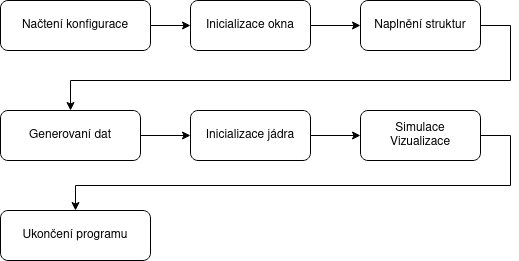
\includegraphics[scale=0.6]{obrazky-figures/Simple.png}
	\caption{\textbf{Základní struktura programu.}}
	\label{fig:simpleStruct}
\end{figure}

Aplikace začíná načtením konfiguračního souboru a inicializací logovacího systému. Konfigurační soubor obsahuje především většinu konstant a parametrů pro správný chod simulace, ale také některé informace týkající se aplikace jako takové. Dalším krokem je inicializace okna schopného zobrazovat simulovaná data převedena do vizuální podoby. Následuje naplnění simulačních struktur a generovaní simulačních dat. Simulační struktury jsou balíčky obsahující statické informace o simulaci, kdežto simulační data obsahují popis konkrétních částí simulace jakožto částic/buňek. Tyto data pak přebírá samotné jádro, které se stará o samotnou simulaci a vizualizaci. Jádro v sobě skrývá simulační moduly pro jednotlivé části simulací, ale zároveň moduly pro vizualizaci výsledků a grafického uživatelského rozhraní. Po inicializaci přihází na řadu samotná simulace a vizualizace. Oba tyto moduly běží v nekonečné smyčce, přičemž vizualizace probíhá každý cyklus, ale výpočty simulace pouze v případě, že je uživatelem simulace spuštěna. Celá tato smyčka trvá tak dlouho, dokud nedojde k ukončení programu uživatelem. V následujících kapitolách jsou tedy jednotlivé části podrobněji rozebrány. 

\section{Konfigurace}
\label{chapter:konfigurace}
Jak je ukázáno na obrázku \ref{fig:simpleStruct}, prvním hlavním krokem celého programu je načtení konfiguračního souboru. Samotná struktura konfiguračního souboru je pak popsána v příloze \ref{appendix:configfile}, nicméně stručně řečeno soubor je rozdělen na několik částí, kde každá část má nějaký svůj určitý význam v celém celku programu. Velkou většinu souboru tvoří především parametry simulace, rozdělené do tří bloků, tedy mřížková metoda, metoda Smoothed Particle Hydrodynamics a nakonec samotné vypařování. Zbývající bloky se pak týkají především nastavení samotné aplikace, jako jsou rozměry okna, cesta k shaderům či třeba poslední pozice a úhel kamery.

Existuje celá řada formátů využívaných pro konfigurační soubory, běžný \texttt{INI}, komplexnější \texttt{YAML}, případně i formáty primáně neurčeny jako konfigurační jako je třeba \texttt{JSON} nebo \texttt{XML}. Nakonec byl však pro účely tohoto projektu zvolen formát \texttt{TOML}. Jedná se o relativně nový formát, který se snaží být čitelný pro běžného člověka, minimalistický a zároveň je vystaven aby byl schopný se snadno mapovat do hašovací tabulky \cite{toml-lang}. Tento formát byl vybrán především kvůli své zvýšené čitelnosti oproti například formátům \texttt{JSON} či \texttt{XML} a to především, protože byly očekávány častější změny v souboru, ale také možnost vyčíst ze souboru současné nastavení simulace. Tohoto bylo využito především v prvotních fázích vývoje, kdy nebyla všechna nastavení propojena do uživatelského rozhraní.

Samotné načtení konfiguračního souboru je pak vcelku primitivní záležitost. K snadnější manipulaci byla využita knihovna \texttt{toml11}, která poskytuje funkce jak pro načítání, tak ukládání konfiguračních souborů. Načtená data jsou pak uložena do třídy \texttt{Config} obsahující struktury \texttt{AppConfig} a \texttt{VulkanConfig}, kde \texttt{AppConfig} je dále rozdělena na další struktury dle jednotlivých simulací. Samotná instance třídy \texttt{Config} je pak různě předávána mezi ostatními částmi programu dle potřeby, přičemž její obsah je využíván k nastavování programu a tvorbě výchozího stavu simulace. Do souboru nejsou propisovány žádné změny udělané v parametrech simulace během používání aplikace, až s vyjímkou pozice kamery. Ta je při ukončení uložena do příslušného načteného souboru, takže po opětovném spuštění aplikace se stejným konfiguračním souborem dojde zároveň k načtení poslední pozice kamery, a uživatel nemusí opět měnit kameru do vhodnější pozice pro daný scénář.

\section{Okno}
\label{chapter:okno}
Jelikož výsledkem této práce je grafická aplikace, která by měla být schopná vizualizovat počítané výsledky uživateli, je nutné vytvořit okno, které je schopné zobrazovat vykreslovaný výstup z použitého API Vulkan. Pro tento účel bylo využito knihovny \texttt{GLFW}, schopné vytvářet okna a plochu pro vykreslování nejen pro v této práci využívaný Vulkan, ale tako OpenGL a OpenGL ES. Dalšími užitečnými vlastnostmi, které \texttt{GLFW} poskytuje je možnost využití různých vstupů jako je námi požadovaná klávesnice a myš, ale zároveň různé časované události, či události samotného okna. Tyto události pak může daná aplikace zpracovávat ve formě tzv. callbacků či pollingu. 

V aplikaci pak byla vytvořena vlastní třída \texttt{GlfwWindow} zapouzdřující funkčnost samotného okna. Kromě poskytování samotného handelu okna pro ostatní třídy, především tedy Vulkan jádra, obsahuje také funkce pro poskytování informací o okně jako jsou jeho rozměry. Hlavní částí je však implementace návrhového vzoru observer. Toto je zabezpečeno děděním od třídy \texttt{EventDispatchinWindow}, která poskytuje funkce pro registraci několika druhů funkcí zpracovávajících události příslušející danému oknu, přesněji události pocházející z klávesnice a myši. Při registraci je funkce uložena do fronty a zároveň je vrácena třída schopná daného posluchače událostí z fronty odstranit. Když následně dojde k vyvolání daného typu událostí jsou všechny funkce přítomné ve frontě zavolány a jako parametr je těmto funkcím předána zpráva obsahující důležitá data o události, jako je například typ klávesy či typ provedené akce. Tyto zprávy pak má za úkol daná funkce zpracovat a adekvátně na ně reagovat například změnou pozice či natočením kamery.


\section{Simulační struktury a simulační data}
\label{chapter:simStructData}
Pro správné fungování simulace je potřeba nejprve vyplnit několik struktur a inicializovat výchozí hodnoty pro částice a mřížkovou metodu. Struktury mající v názvu \enquote{Info} jsou pak statické struktury které se v čase nemění, pouze na popud uživatele, který mění parametry simulace. ostatní jsou datové struktury držící stav simulace a měnící hodnoty v jejím průběhu.

\subsubsection{Smoothed Particle Hydrodynamics}
Stav jednotlivých částic představuje pole sestávající se z několika struktur popsaných na obrázku \ref{fig:ParticleRecord}. Výchozí pozice pro částice jsou pak generovány v závislosti na objemu kapaliny, velikosti daného modelu a počáteční pozici. Důležité je upozornit, že generování nebere v potaz pozici a velikost simulovaného prostoru a proto při špatném konfiguračním souboru může dojít k destabilizaci simulace.  Dále budou popsány pouze komponenty, které nemusí být na první pohled zřejmé, co představují. 

Struktura obsahuje dvakrát hodnotu rychlosti, nicméně nejedná se o duplicitní hodnoty, ale přítomnost obou dvou vyplývá z implementace algoritmu Leap-frog popsaném v kapitole \ref{chapter:SPH}. V tomto algoritmu, dochází totiž k střídavému výpočtu mezi rychlostí a pozicí, pozice je vždy vychází z pozice v čase $t-1$ a dostáváme pozici v čase $t$. U rychlosti ale nastává problém, ta vychází z pozice v čase $t-\frac{1}{2}$ a dostáváme pozici v čase $t+\frac{1}{2}$. Z toho vyplývá, že abychom byly konzistentní potřebujeme pro další výpočty využívat rychlost v čase $t$ tedy parametr \texttt{currentVelocity}, nicméně pro výpočet následující rychlosti $u_{t+\frac{1}{2}}$ je nutné vycházet z předešlé rychlosti $u_{t-\frac{1}{2}}$ tu pak reprezentuje část \texttt{velocity}. Parametry \texttt{massDensityCenter} a \texttt{weightingKernelFraction} jsou pomocné parametry sloužící k předávání informací mezi jednotlivými částmi simulace pro výpočet povrchu, který částice zaujímá v celkovém objemu. Část \texttt{dummy} pak představuje hodnotu především pro testovací účely schopnou ukládat různá data a položka \texttt{gridID} je příslušnost částice k buňce v simulaci v rámci urychlení vyhledávání sousedů.

\begin{figure}[h]
	\centering
	\begin{subfigure}[t]{.5\textwidth}
			\centering
        	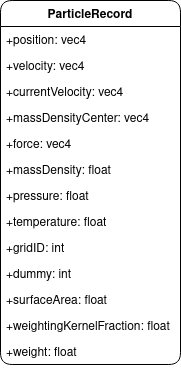
\includegraphics[scale=0.6]{obrazky-figures/ParticleRecord.png}
        	\caption{\textbf{Struktura představující částici}}
        	\label{fig:ParticleRecord}
	\end{subfigure}%
	\begin{subfigure}[t]{.5\textwidth}
		\centering
		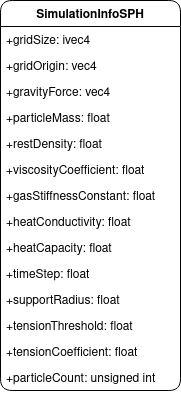
\includegraphics[scale=0.6]{obrazky-figures/SimulationInfoSPH.png}
		\caption{\textbf{Informační struktura}}
		\label{fig:SimInfoSPH}
	\end{subfigure}
	\caption{Simulační struktura a simulační data pro SPH simulaci.}
	\label{fig:structsSPH}
\end{figure}

\newpage

Informační struktura \ref{fig:SimInfoSPH} je pak vcelku zřejmá a většina parametrů je naplněna z konfiguračního souboru. Za zmínku snad stojí pouze výpočet vyhlazovacího poloměru, který vychází z následujícího vzorce
\begin{equation}
    h=\sqrt[3]{\frac{3 V x}{4 \pi n}}
\end{equation}

kde $x$ představuje přibližný počet částic obsažených v poloměru a $n$ je celkový počet částic.


\subsubsection{Mřížková metoda}
Mřížková metoda má minimum hůře pochopitelných částí. Jednou z nich je však parametr \texttt{specificInfo}, který je vytvořen tak, že v závislosti na současném průběhu simulace nese jiné informace. Reálně je však využit pouze při výpočtu difuze a divergence. V těchto krocích je totiž využito Gauss-Seidlova numerického algoritmu, který je však nevhodný pro paralelní systémy a proto je využito paralelní verze toho algoritmu a zmíněný parametr nese specifické informace potřebné pro daný algoritmus. Parametry \texttt{bouyancyAlpha} a \texttt{bouyancyBeta} pak představují konstanty $\alpha$ a $\beta$ ve vzorci \ref{eq:buoyEvap}.

Samotné data nesoucí stav simulace jsou pak uloženy v samostatných polích. Existuje tedy pole nesoucí rychlosti v daných buňkách a pole nesoucí informace o hustotě a teplotě dané buňky. K tomuto rozdělení došlo především z důvodu mnoha kroků simulace a tedy k častému užití pouze části dat. Obě pole jsou pak duplikovány, a to z důvodu nutnosti využití předešlých hodnot při výpočtu nových hodnot. 

\begin{figure}[hbt]
	\centering
	\captionsetup{justification=centering}
	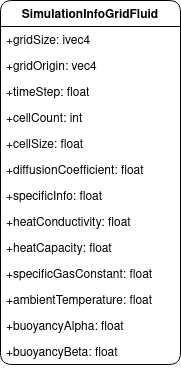
\includegraphics[scale=0.6]{obrazky-figures/SimulationInfoGridFluid.png}
	\caption{\textbf{Informační struktura pro mřížkovou metodu}}
	\label{fig:structsGrid}
\end{figure}

\subsubsection{Vypařování}
jelikož vypařování funguje na principu propojení obou typů simulací, je logické, že v informační struktuře zobrazené na obrázku \ref{fig:structsEvap} jsou obsaženy informace jak o částicové simulaci, tak o mřížkové. Parametry \texttt{coefficientA} a \texttt{coefficientB} jsou pak konstanty ve vzorci \ref{eq:EvapRate} ovlivňující rychlost vypařování. Jelikož simulace vypařování pracuje jak s částicemi tak s buňkami, je nutné samozřejmě využít i pole částic z částicové simulace a pole rychlostí, hustot a teplot z mřížkové simulace.

\begin{figure}[hbt]
	\centering
	\captionsetup{justification=centering}
	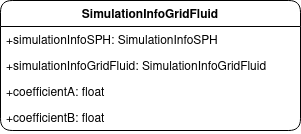
\includegraphics[scale=0.6]{obrazky-figures/SimulationInfo.png}
	\caption{\textbf{Informační struktura pro simulaci vypařování}}
	\label{fig:structsEvap}
\end{figure}


\section{Jádro}
\label{chapter:jadro}

Jádro simulace je hlavním středobodem celé aplikace. Jedná se o třídu \texttt{VulkanCore}, které se stará nejen o inicializaci jednotlivých simulačních modulů, ale také o jejich správné spouštění, synchronizaci a inicializaci celého Vulkan API. Tato třída byla prvotně implementována na základě návodu \footnote{\url{https://vulkan-tutorial.com/}}, pomocí které byla vytvořena prvotní kostra aplikace a došlo k seznámení se samotným API Vulkanu. K samotné implementaci však bylo využito rozhraní v jazyku C++, místo v návodu zmiňovanému C. Hlavičkový soubor \texttt{vulkan.hpp} totiž oproti jeho C verzi přináší několik nesporných výhod, kde mezi největší lze zařadit využití výčtových typů místo maker a využití \texttt{UniqueHandle} pro automatickou správu objektů. 

V průběhu tvorby tohoto jádra pak docházelo k postupnému přesouvání důležitých komponent do vlastních tříd, s tím že každá třída dostala několik funkcí pro snadnější manipulaci s jejími součástmi. Navíc pro složitější komponenty jako například \texttt{Pipieline}, \texttt{Buffer}, či \texttt{Image}, byly vytvořeny \enquote{\texttt{Builder}} třídy usnadňující tvorbu komponenty. Není tak nutné vytvářet složité konstruktory a plnit často obrovské struktury, pro vytvoření stačí konstruktoru předat inicializovaný \texttt{Builder} s několika málo dalšími komponenty. Tento přístup má nespornou výhodu při vytváření několika podobných objektů, lze tak vytvořit jeden \texttt{Builder} objekt a ten pak jen lehce upravovat před použitím v každém konkrétním objektu.

\subsection{Uživatelské rozhraní}
\label{chapter:uzivRozh}

Důležitou součástí celého jádra je pak instance třídy \texttt{SimulationUI}. Ta se stará o inicializaci, vykreslování, ale i zpracování událostí v rámci grafického uživatelského rozhraní. Celé rozhraní je pak vytvořeno za pomocí knihovny \texttt{pf\_imgui} \footnote{\url{https://github.com/PetrFlajsingr/pf_imgui}} založené na knihovně \texttt{Dear ImGui} \footnote{\url{https://github.com/ocornut/imgui}}. Knihovna \texttt{pf\_imgui} je stále ve vývoji a je vyvýjena studentem Fakulty informačních technologií. V tomto projektu je využívána ve verzi v0.4.2 a je používána především kvůli zjednodušení tvorby a správy jednotlivých komponent. Celé rozhraní je detailněji popsáno v příloze \ref{appendix:gui}, avšak stručně řečeno celé uživatelské rozhraní je obsaženo v jednom okně, které je rozděleno do panelů schopných skrývat svůj obsah. V těchto panelech pak uživatel může libovolně měnit nastavení simulace, případně ji ovládat či nahrávat.

\begin{figure}[hbt]
	\centering
	\captionsetup{justification=centering}
	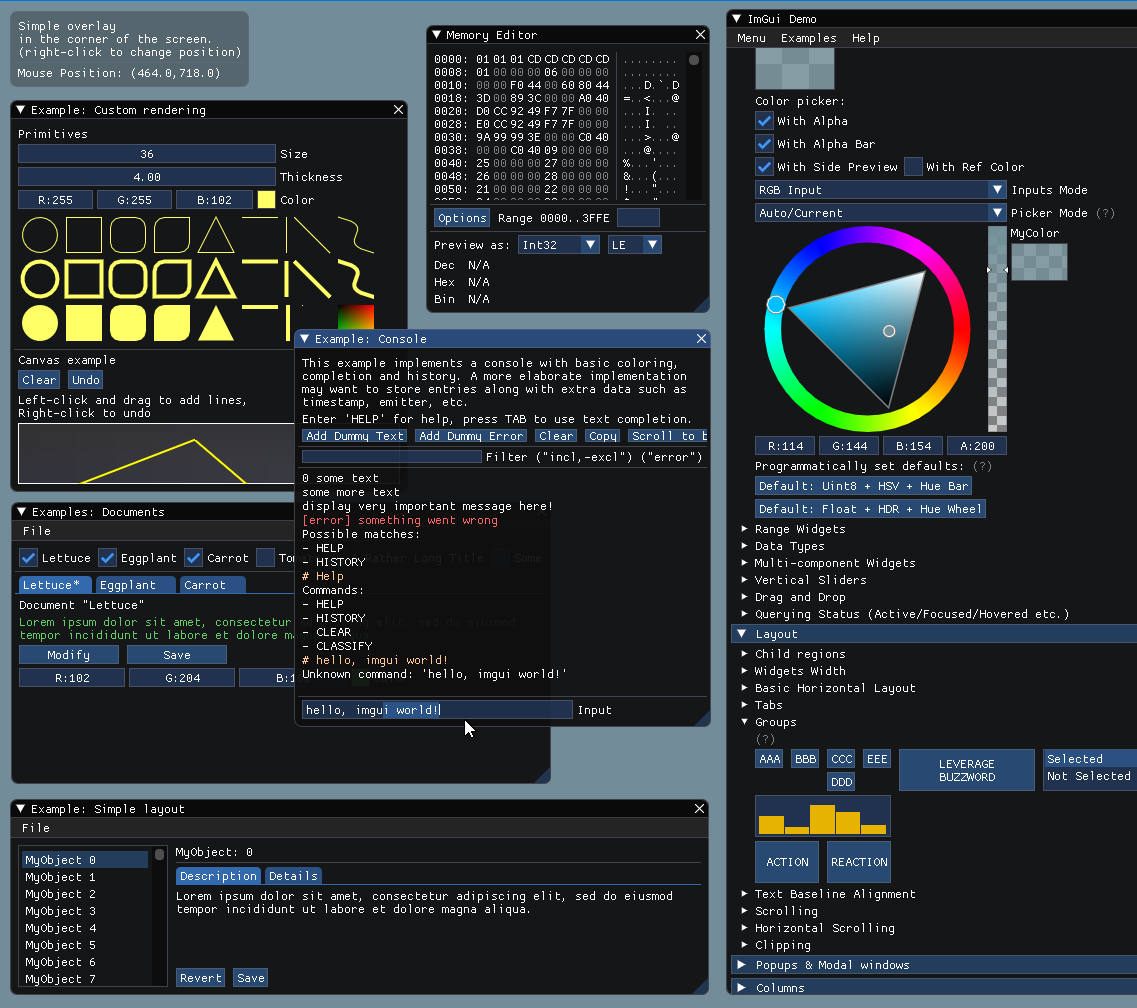
\includegraphics[scale=0.2]{obrazky-figures/imgui.png}
	\caption{\textbf{Dear ImGui.} Demostrační aplikace představující knihovnu ImGui.}
	\textbf{Zdroj: } \url{https://github.com/ocornut/imgui}
	\label{fig:structsEvap}
\end{figure}

Před vytvářením samotných komponent, je nutné instanci zmíněné třídy představující uživatelské rozhraní naplnit potřebnými komponentami jako je například samotné okno či zařízení nebo instance Vulkanu. Dalším důležitým krokem je nahrát vyplněné struktury popsané v kapitole \ref{chapter:simStructData}. Díky tomu je zajištěna konzistence informací pro simulaci a zobrazených údajů pro uživatele. Následně může dojít k samotné tvorbě komponent. Tyto komponenty pak načítají výchozí data ze zmíněných struktur. Důležitou součástí je i reaktivnost aplikace tedy propojení akce provedené v grafickém rozhraní do samotné simulace. Toto je zajištěno voláním příslušných funkcí z třídy rozhraní. Máme-li například tlačítko pojmenované \texttt{buttonStartSimulation}, je volán odkaz na funkci se jménem \texttt{onButtonStartSimulationClick()}. Tyto odkazy na funkce jsou pak naplňovány tzv. \enquote{settery}. Společně se zavoláním příslušné funkce je také z třídy \texttt{SimulationUI} často předán parametr obsahující důležitá data vztahující se k dané akci. Taková data pak mohou představovat například vybranou barvu, či výčtový typ označující vybranou položku z rolovacího menu. Pomocí takového volání funkcí a předávání zprav je zajištěná komunikace mezi grafickým rozhraním a samotným jádrem aplikace.

\section{Simulace}
\label{chapter:simulace}
Simulace je hlavní částí celé aplikace. Samotné řízení simulace probíhá z již zmíněné instance třídy \texttt{VulkanCore}, nicméně sama třída neprovádí žádnou simulaci, ale pouze spouští příslušné moduly odpovídající jednotlivým typům simulace. Veškeré algoritmy jsou pak spouštěny na grafické kartě z důvodu urychlení. Na obrázku \ref{fig:simflow} lze vidět průběh jednoho kroku celé aplikace včetně vizualizace. Samotná simulace je pak běží pouze v případě, že ji uživatel spustil, případně si vyžádal pouze jeden další krok simulace. Za zmínku pak stojí jistě blok nazvaný \enquote{Inicializace SPH}. Tento blok provádí částečný výpočet částicové simulace a je nezbytný pro správné zobrazování povrchu kapaliny při metodě Marching cubes. Jelikož daná metoda spoléhá na určité vypočítané hodnoty, je nutné je předpočítat, jinak by nebyl produkovát korektní výsledek při výchozím stavu celého simulátoru.

\begin{figure}[h]
	\centering
	\begin{subfigure}[t]{.5\textwidth}
			\centering
        	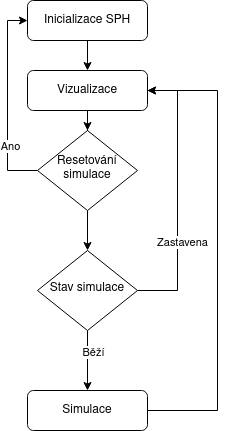
\includegraphics[scale=0.6]{obrazky-figures/SimFlow.png}
        	\caption{\textbf{Zobecněný postup při simulaci}}
        	\label{fig:simflow}
	\end{subfigure}%
	\begin{subfigure}[t]{.5\textwidth}
		\centering
		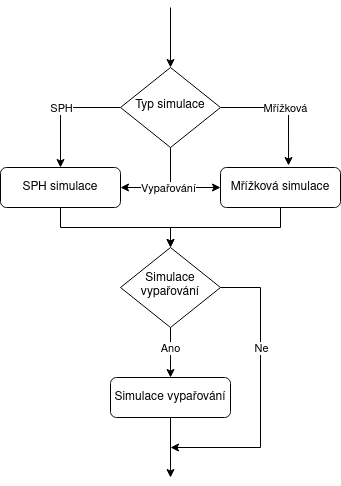
\includegraphics[scale=0.6]{obrazky-figures/SimTypeFLow.png}
		\caption{\textbf{Detail bloku Simulace z obrázku \ref{fig:simflow}}}
		\label{fig:simTypeflow}
	\end{subfigure}
	\caption{Tok programu při simulaci}
	\label{fig:SimulationFlow}
\end{figure}

Na obrázku \ref{fig:simTypeflow} je pak detailněji zobrazen blok samotné simulace a rozhodování, která simulace bude zrovna prováděna. Dochází-li ke kombinované simulaci, tedy k simulaci vypařování, jsou nejprve současně spuštěny obě simulace, simulace částicová (v obrázku SPH) a mřížková. Tyto simulace lze spustit současně, jelikož se jedná o nezávislé výpočty, tudíž mohou lépe zaplnit výpočetní prostor samotné grafické karty a ušetřit nějaký čas. Před samotným výpočtem vypařování je však nutné tyto procesy synchronizovat a počkat až oba doběhnou. následně se pokračuje do grafu \ref{fig:simflow} a dochází k vizualizaci výsledku.



\subsection{Smoothed particle hydrodynamics}
\label{chapter:simSPH}

\begin{figure}[hbt]
	\centering
	\captionsetup{justification=centering}
	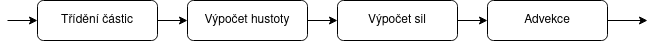
\includegraphics[scale=0.6]{obrazky-figures/SPH.png}
	\caption{\textbf{SPH simulace} Jednotlivé kroky SPH simulace.}
	\label{fig:SPHflow}
\end{figure}

Částicová simulace vychází z algoritmu popsaném v kapitole \ref{chapter:SPH} vycházejícího z publikace \cite{KelagerSPH} Mickyho Kelagera z University of Copenhagen. Tento algoritmus je představován především bloky \textit{Výpočet hustoty}, \textit{Výpočet sil} a \textit{Advekce} z obrázku \ref{fig:SPHflow}. Jediný blok který je dále rozdělený na více částí je blok s výpočtem hustoty částice. Zde je ještě proveden výpočet středu hustoty, který vychází z článku \cite{sufaceSPH}. Tento výpočet je nezbytný, jelikož velikost plochy která částice zaujímá v kapalině ovlivňuje výpočet míry vypařování. Rozdělení do těchto bloků je pak dáno především závislostí výpočtů, jelikož většina výpočtů v bloku \textit{Výpočet sil} k výpočtu vyžaduje současnou hodnotu hustoty částic, je zapotřebí ji nejprve vypočítat pro všechny částice a až následně přejít k dalším výpočtům.

\subsubsection{Urychlení vyhledávání}
pro výpočet nových hodnot částice během simulace je z principu rovnice \ref{eq:SPHsum} nutné počítat se všemi částicemi v okolí. Nicméně ne všechny částice nutně přispívají k celkovému výsledku. Částice nacházející se ve vzdálenosti větší než je vyhlazovací poloměr $h$ nepřispívají k výpočtu. Při nízkém počtu částic se nejedná o nijak závažný problém, avšak při vysokém počtu částic dochází k tomu, že při výpočtu procházíme například desetitisíce částic, ale k samotnému výpočtu přispěje pouze několik málo desítek částic. 

Z tohoto důvodu je jeví jako více než vhodné, využít metody schopné získat pouze částice přispívající k výpočtu hodnot. Autor publikace \cite{KelagerSPH} navrhuje využití prostorového hešování, nicméně tento postup byl odmítnut ve prospěch homogenní mřížky. Hlavním důvodem byla možnost snadnější propojení s mřížkovou metodou simulace. Tato metoda sice neomezuje průchod pouze na částice spadající pod velikost vyhlazovacího poloměru, nicméně výrazně redukuje počet částic, se kterými je nutné počítat. Princip metody je zobrazen na obrázku \ref{fig:GridSPH}. Principem je rozdělení částic do mřížky, kde každá buňka má velikost rovnou vyhlazovacímu poloměru. Pokud tedy počítáme s Moorovým okolím, máme zajištěno, že částice nacházející se v tomto okolí jsou množinou obsahující všechny částice potřebné k výpočtům. Na samotném obrázku je pak modře znázorněna částice, pro kterou jsou hodnoty počítány, zelené jsou částice potřebné pro výpočet a červené částice, které budou zahrnuty do výpočtu, ale nejsou potřebné. Oranžový kruh pak znázorňuje vyhlazovací poloměr.

\begin{figure}[hbt]
	\centering
	\captionsetup{justification=centering}
	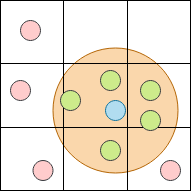
\includegraphics[scale=0.6]{obrazky-figures/GridSPH.png}
	\caption{\textbf{Mřížková metoda pro urychlení vyhledávání}}
	\label{fig:GridSPH}
\end{figure}

Celý průběh takového algoritmu pak probíhá následovně. Nejprve je dle pozice vypočtena příslušnost částice k buňce. Tato informace je zapsána do separátního pole společně s pořadovým číslem částice. Následně je využito paralelního řazení a celé toto pole indexů částic a buněk je seřazena dle indexu buňky. Pro řazení byl zvolen algoritmus Count sort \cite{CountSortGPU} využívající algoritmu prefix sum \cite{GPUGemsPrefixSum}.  Výsledkem je tedy seřazená posloupnost, přičemž indexy částic ve stejné buňce se nacházejí za sebou. Posledním krokem je pak tvorba dalšího pole s indexy ukazujícím na začátek jednotlivých bloků buněk. Takový index nám pak ukáže kde se nachází konkrétní buňka s částicemi. Pokud je buňka prázdná, obsahuje speciální hodnotu -1 značící prázdnost. Při následném prohledávání okolí při výpočtech pak stačí znát pouze index buňky, který označí seznam příslušných částic.

\subsection{Mřížková simulace}
\label{chapter:simGrid}
Další součást obrázku \ref{fig:simTypeflow} nutnou popsat je mřížková metoda simulace, které je zobrazena na obrázku \ref{fig:Gridflow}. Tu lze rozdělit na dvě části skládající se následovně z několika dalších kroků. Dva hlavní bloky představují rychlost a hustotu s teplotou. Obě části pak mají stejné kroky a proto budou vysvětleny obecně, přičemž však budou popsány případné jednotlivé odlišnosti.

\begin{figure}[hbt]
	\centering
	\captionsetup{justification=centering}
	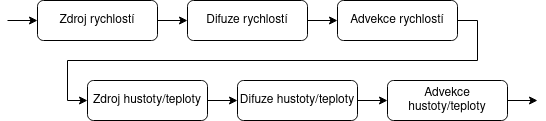
\includegraphics[scale=0.6]{obrazky-figures/GridFluid.png}
	\caption{\textbf{Mřížková simulace} Jednotlivé kroky mřížkové simulace.}
	\label{fig:Gridflow}
\end{figure}

Blok Zdrojů je poměrně jednoduchý a dochází v něm pouze k přidávání hodnot do jednotlivých částí, jedná se tedy o určité působení okolních zdrojů. Do pole rychlostí se následně ještě připočítává působení hustoty a teploty podle vzorce \ref{eq:buoyEvap}. Následně je přistoupeno k difuzi, kdy dochází k rozptýlení hodnot do okolí. V tomto případě však může dojít k vzniku nenulové divergence a proto je nutné aplikovat projekci a tuto divergenci odstranit případně minimalizovat, čehož dosahuje za pomocí Gauss-Seidlovy numerické metody, využívané i při výpočtu difuze. Posledním krokem je pak advekce, která je implementována pomocí tzv. backtrackingu popsaném v kapitole \ref{chapter:Grid}. Advekce hodnot hustoty a teploty pak využívá již vypočtených hodnot rychlosti a je tak nutné vyčkat s výpočtem na advekci rychlostí.

Problém nastává při aplikování Gauss-Seidlovy numerické metody. Principem této metody je průchod pole a postupný výpočet nových hodnot tak jak je to znázorněno na obrázku \ref{fig:GaussSeidl}, kde červeně jsou pak označeny již vypočtené hodnoty a černé šipky označují ze kterých hodnot se nová hodnota počítá. Tento postup je však neproveditelný na paralelních architekturách, proto musel být zvolen jiný přístup. Vhodnější metodou je tedy využití algoritmu Gauss-Seidel Red Black \cite{Amador2012LinearSF}. Tento přístup využívá střídavého počítání hodnot v červených a černých bodech zobrazených na obrázku \ref{fig:GaussSeildRB}. Tím je docíleno, že jsou na sobě závislé pouze kroky střídání barev a lze tedy využít pro výpočet paralelní architekturu. Tato metoda sice vyžaduje podle autorů článku \cite{Amador2012LinearSF} dvojnásobný počet iterací pro správnou konvergenci, nicméně pro větší počet buněk dochází k výraznému urychlení díky právě paralelním výpočtům.

\begin{figure}[h]
	\centering
	\begin{subfigure}[t]{.5\textwidth}
			\centering
        	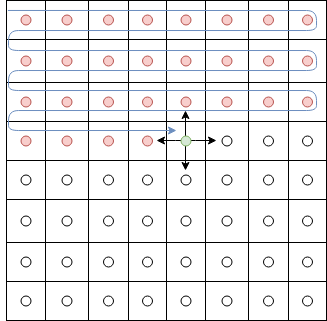
\includegraphics[scale=0.5]{obrazky-figures/Gauss.png}
        	\caption{\textbf{Gauss-Seidlova numerická metoda}}
        	\label{fig:GaussSeidl}
	\end{subfigure}%
	\begin{subfigure}[t]{.5\textwidth}
		\centering
		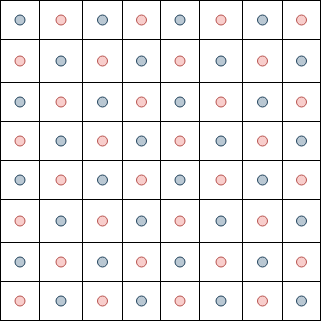
\includegraphics[scale=0.5]{obrazky-figures/GaussRB.png}
		\caption{\textbf{Paralelní verze Gauss-Seidlovy Metody}}
		\label{fig:GaussSeildRB}
	\end{subfigure}
	\caption{Tok programu při simulaci}
	\label{fig:numGauss}
\end{figure}

V samotné aplikaci je pak invokován stále stejný výpočetní shader, avšak je využito právě specifické informace ve struktuře \ref{fig:structsGrid}. Ta poté představuje bitové pole nesoucí mimo jiné informaci po barvě právě prováděné iteraci. Díky této informaci jsou pa upraveny indexy pro přístup do pole hodnot.

\subsection{Vypařování}
\label{chapter:simEvap}

\begin{figure}[hbt]
	\centering
	\captionsetup{justification=centering}
	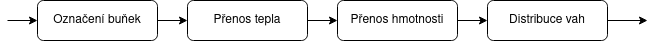
\includegraphics[scale=0.6]{obrazky-figures/EvapFlow.png}
	\caption{\textbf{Simulace vypařování} Jednotlivé kroky simulace vypařování.}
	\label{fig:EvapFlow}
\end{figure}

Poslední částí je simulace vypařování, k té však dochází pouze po kompletním výpočtu kroku předchozích dvou simulací. Samotná simulace je pak zobrazena na diagramu \ref{fig:EvapFlow}. Důležitou součástí celého procesu je označení jednotlivých buněk. Každá buňka pak dostane dvě značky nesoucí informace o buňce. První je, zda se jedná o buňku obsahující částice. Během simulace vypařování dochází k přenosu hmotností mezi částicovou simulací a simulací mřížkovou. Označením, zda buňce náleží nějaká část kapaliny, můžeme následně zamezit vypařování do míst obsahujících kapalinu. Druhou značkou přiřazenou buňkám v první části simulace je zda se jedná o rozhraní mezi kapalinou a okolím. Buńka je vyhodnocena jako rozhraní, jedná-li se o buňku mající ve svém nejbližším okolí buňku jiného typu, tedy buňku prázdnou či obsahující kapalinu. Jako bylo zvoleno trojrozměrné Von-Neumanovo okolí, kde jeho dvojrozměrná verze je zobrazena na obrázku \ref{fig:neighbours}. Takto vzniká označení rozhraní na obou stranách povrchu kapaliny. Toto označení je důležité z hlediska přenosu tepla mezi kapalinou a okolím, jelikož přenos tepla nastává pouze na povrchu kapaliny. 

Samotný blok přenosu tepla se pak v aplikaci rozděluje na přenos tepla z kapaliny do okolí a z okolí do kapaliny. Samotný přenos hmotnosti pak funguje pouze jednosměrně a využívá váhových faktorů zmíněných v na konci kapitoly \ref{chapter:evap}. Na konci simulace pak dochází k vyrovnávání zmíněných faktorů. Existuje-li částici s váhou $w < 0.5$ dochází k jejímu zániku a distribuci její zbylé váhy do okolních částic. Využití těchto vah spolu nese nutnost začlenit tyto váhy do výpočtů samotné částicové simulace, ale také v ostatních částech simulace, kde částice s váhou $w = 0$ tedy zaniklé částice, nejsou brány v potaz při výpočtu výsledku. Příkladem může být například zmíněné značení buněk.

\section{Vizualizace}
\label{chapter:Vizualizace}
Důležitou součástí celé aplikace je také vizualizace výsledku simulace, bez ktéré by výsledkem byla jen změť pozic, rychlostí a jiných hodnot. Vizualizaci je nutné provádět jak pro částicovou simulaci, tak pro simulaci mřížkovou, níže jsou pak popsány použité metody pro zobrazování jednotlivých simulací.

\subsection{Smoothed particle hydrodynamics}
\label{chapter:vizSPH}
Ve vytvářené aplikaci byly použity metody přímé vizualizace částic a extrakci povrchu pomocí Marching cubes. Mezi těmito metodami lze následně libovolně přepínat. Důležitou součástí je také možnost vizualizace hustoty jednotlivých částic pomocí barevného rozložení.

\subsubsection{Vizualizace částic}
Vizualizace částic je tou nejprimitivnější metodou vizualizace schopnou vykreslit jednotlivé částice, jedná se o poměrně nenáročnou metodu schopnou zobrazovat jednotlivé výpočetní částice v kapalině. Hlavním principem je pak technika instancovaného vykreslování. V paměti grafické karty je tak uložen jeden model a ten je následně vykreslován několikrát za sebou tak aby počet odpovídal počtu částicím. Na každou jednotlivou instanci modelu je pak aplikována translace a škálování tak aby daná instance odpovídala pozici konkrétní částice a její váze $w$.

tento typ vykreslování byl implementován již na začátku celého vývoje a jeho nespornou výhodou je možnost sledovat chování jednotlivých částic. Zvolený model koule pak má výhodu totální symetrie a tedy odpadá nutnost určitým způsobem rotovat části, aby působila dojmem reálného pohybu, jako by tomu bylo například u krychle.

\subsubsection{Marching cubes}
Metoda Marching cubes \cite{marchingCubes} je metoda extrakce povrchu za pomocí předem definované funkci, tzv. signed distance function. Daná funkce nám dokáže říci, na jaké straně objektu se nacházíme a jaké je vzdálenost k jeho povrchu. Pomocí ní pak dokážeme navzorkovat daný prostor rozdělený do mřížky a v každém vrcholu buňky mít hodnotu o vzdálenosti k povrchu. Buňkami které následně neleží čistě vně či uvnitř objektu prochází povrch daného modelu. V průběhu let pak bylo vytvořeno několik modifikací vyhledávacích tabulek určujících jaké hrany buňky propojit, aby výsledkem byl \enquote{vodotěsný} model aproximující danou funkci.

\begin{figure}[hbt]
	\centering
	\captionsetup{justification=centering}
	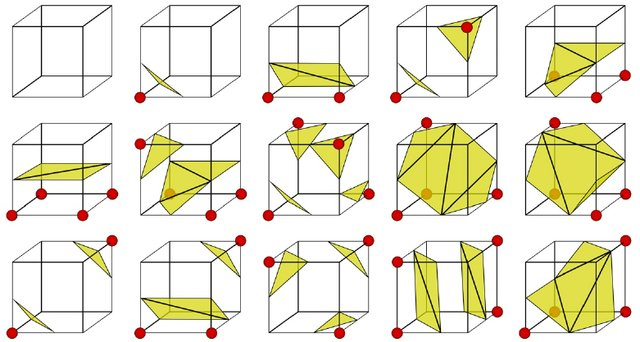
\includegraphics[scale=0.5]{obrazky-figures/Look-up-table-for-the-Marching-Cubes-algorithm-13_W640.jpg}
	\caption{\textbf{Vyhledávací tabulka Marching cubes} Červeně jsou označeny body uvnitř modelu.}
	\textbf{Zdroj: } Isovox: A Brick-Octree Approach to Indirect Visualization \cite{isovox}
	\label{fig:EvapFlow}
\end{figure}

V samotné aplikaci je pak algoritmus řešen pomocí výpočetních a geometrických shaderů. Výchozí velikost mřížky je stejná jako je velikost mřížky pro usnadnění vyhledávání popsané v kapitole \ref{chapter:simSPH}. Výchozí mřížka je však velmi hrubá a produkuje poměrně hrubý model. Z toho důvodu je možnost zvýšit detail výsledného modelu pomocí rozdělení každé buňky na několik dalších, čím je docíleno jemnějšího vzorkování při výpočtu a následně detailnějšího modelu. Pro vzorkování je pak využita funkce výpočtu barevného pole \ref{eq:ColorField}, přičemž jako práh rozdílu mezi kapalinou a okolím byla zvolena hodnota 0,5.

Při samotném vykreslování pak dochází opět k instancovanému vykreslování, nicméně nyní se jedná pouze o body představující jednotlivé buňky. do vykreslovacího toku je pak zařazen geometrický shader, který dle navzorkované mřížky a kompletní vyhledávací tabulky produkuje polygony představující povrch kapaliny.

\subsection{Mřížková simulace}
\label{chapter:vizGrid}
Prvním pokusem pro mřížkovou simulaci především pro testování bylo obdobné renderování jako je vizualizace částic. V tomto případě však došlo k instancovanému renderování krychlí černé barvy. Každá krychle pak měla nastavenou průhlednost v závislosti na množství obsažené v dané buňce. Různě průhledné buňky byly následně míchány mezi sebou a vznikala iluze kouře. Bohužel tato iluze nebyla dostatečně věrná a proto bylo přistoupeno k jiné metodě.

Výsledná použitá metoda je pak modifikací na vykreslování zmíněné ve článku Visual Simulation of Smoke \cite{visualSmoke}. Každá buňka obsahující nějaké množství látky je pak renderována jako čtverec zarovnaný s osou, která je nejvíce paralelní s osou pozorovatele. Následně jsou čtverce vykresleny, nicméně každý vrchol je brán jako jiná buňka a tak dochází k interpolaci průhledností mezi jednotlivými vrcholy. Jedná se o v celku jednoduchou techniku, která ale produkuje v celku působivé výsledky.

\chapter{Testování}
\label{chapter:testovani}
Chod celého simulátoru byl testován především během vývoje. Po přidání nové funkčnosti jako je například nový způsob vizualizace, případně nový modul pro simulaci, byl otestován chod nejen současného modulu, ale i stávajících součástí systému. Po přidání modulu, případně refaktorizaci kódu totiž často docházelo k porušení synchronizace mezi jednotlivými invokacemi výpočtů. Výsledná aplikace se tak často stala částečně ale někdy úplně nefunkční. V těchto případech však byly velmi nápomocné validační vrstvy Vulkanu. Tyto vrstvy pak hlásily nejen kritické chyby zapřičiňující zamrzání či pád aplikace, ale také nesprávné používání samotného API a tedy možné snížení výkonu.

Samotné testování a ladění aplikace bylo často velmi komplikované. Ladit v aplikaci strnu běžící na klasickém procesoru byla v celku běžná záležitost krokování a zkoumání hodnot proměnných. Avšak ladění výpočtů běžících na grafické kartě bylo o poznání složitější. Programátor nemá možnost kdykoliv nahlédnout do obsahu paměti a nemá možnost ani spuštěný výpočet v libovolný okamžik zastavit. Proto bylo implementováno několik funkcí, které měli tento proces usnadnit. Jedním s hlavních pomocníků byla funkce čtení paměti z grafické karty. Často tak bylo postupováno tak, že byl program zastaven ihned po dokončení výpočtu a přenesení dat z grafické karty do paměti počítače. Zároveň byly v záznamech částic vytvářeny pomocné proměnné do kterých byly ukládány mezivýsledky. Výraznou pomocí pak byl objev rozšíření \texttt{GL\_EXT\_debug\_printf}. Toto rozšíření po správném nastavení umožňuje diagnostický výpis přímo z grafické karty do validačních vrstev. Tohoto přístupu bylo následně hojně využíváno a společně s předešlou možností nahlédnutí do paměti, tvořili dostatečný způsob ladění celé aplikace.

Každá simulace pak byla otestována s různými velikostmi simulačních prostorů. Pro ladění a hledání chyb bylo často využíváno malého počtu částic případně buněk. To pomohlo v snadnější orientaci ve výpisech a umožňovalo i případné ruční nákresy či výpočty. po odladění na malém prostoru byl algoritmus také otestován na větších objemech a případně laděn dál. Jelikož velké množství simulace se odehrává na homogenní mřížkou, byl velice nápomocný čtverečkovaný papír, kde bylo možné jednotlivé situace rozkreslit a zapsat si například jednotlivé indexy a přemýšlet na řešením problému.

\subsubsection{Smoothed particle hydrodynamics}
Největším problémem této metody bylo nalezení správných parametrů simulace. Ačkoliv byl algoritmus správný, se špatnou kombinací parametrů jako je například dlouhý krok simulace a vysoká viskozita dojde k nestabilitě simulace. Dalším velkým problémem bylo výchozí postavení částic. Pokud byly částice natěsnány velmi blízko u sebe, došlo v prvním kroku simulace k výpočtu velmi vysoké hustoty jednotlivých částic a s tím spojeným vysokým tlakem. Pomocí těchto hodnot byla následně vypočtena rychlost tak aby neprodleně redukovali tlak a hustotu na hodnoty odpovídající dané kapalině. Z toho důvodu byla vypočítaná rychlost velmi vysoká a reálně docházelo k \enquote{explozi} dané kapaliny. Při opačném stav, kdy byly částice velmi daleko od sebe docházelo k vyrovnání hodnot tak, že celý model \enquote{implodoval} a opět se simulace stala nestabilní.

\subsubsection{Mřížková simulace}
Testovat mřížkovou simulaci bylo velmi obtížné z důvodu mnoha kroků simulace. Najít krok kde se nachází chyba bylo obtížné a bylo velmi obtížné interpretovat správnost výstupů ve formě vektorů rychlosti a hodnot teploty a hustoty. Nápomocná však byla již hotová funkční implementace \footnote{\url{https://github.com/BlainMaguire/3dfluid}}. S touto implementací byly pak srovnávány výsledky jednotlivých kroků a pokud byly v rámci mezí, bylo přistoupeno k testování dalšího kroku.

Další důležitou částí, která dělala problém byl výpočet správnosti používaných indexů, především pak při paralelní Gauss-Seidlově metodě, kde je nutné indexovat pouze některé buňky. Zde bylo velmi nápomocné testovat a ladit danou část nad malým počtem buněk, rozepsat si jednotlivé indexy a zjišťovat nesrovnalosti ve výpočtech.


\chapter{Závěr}
\label{chapter:zaver}

Cílem celé práce bylo vytvořit aplikaci schopnou simulovat chování kapaliny a tím se seznámit s principy simulování kapalin. K dosažení tohoto cíle bylo nutné nejdříve nastudovat jednotlivé algoritmy. Toto studium se pak sestávalo nejen ze studia algoritmů které byly následně implementovány, ale také jiných metod pomocí níž lze simulovat chování kapalin.

Následný návrh se nadále zabýval nejen samotnou funkčností aplikace, ale bylo také stanoveno, že projekt bude implementovat dva různé přístupy k simulaci a tedy metodu Smoothed Particle Hydrodynamics a Eulerovu mřížkovou metodu. Současně byl vybrán článek \cite{Evap&Cond} zaměřující se na vypařování a kondenzaci propojením těchto dvou metod. Celý článek byl nastudován a byly zde představeny jeho principy a rovnice nutné k jeho implementaci. Zároveň bylo řečeno, že nedojde k implementaci obou jevů, nýbrž bude implementováno pouze vypařování. Další důležitou součástí návrhu byl pak výběr grafického API, využitého při následné Implementaci. Bylo vybíráno z několika kandidátů, přičemž každý byl krátce rozebrán, byly zmíněny jeho výhody a nevýhody a na konci byl učiněn finální výběr. Jako výsledné API byl zvolen Vulkan, především pro jeho rostoucí popularitu a kontrolu kterou programátorovi nabízí. Poslední částí návrhu pak byl návrh grafického rozhraní. Zde byly navrhnuty ovládací prvky pro celou aplikaci, které uživateli usnadní používání celé aplikace.

Pro implementaci pak bylo využito zmíněného API Vulkan, pomocí kterého bylo dosaženo plné simulace na grafické kartě a využití tak paralelního potenciálu celého problému. Během implementace však bylo nutné řešit řadu problémů, především nutnost studia některých paralelních algoritmů, jelikož některé články poskytovaly algoritmy nevhodné pro paralelní architektury.

Výsledná aplikace je funkční a produkuje uspokojivé výsledky, nicméně se zdaleka nejedná o dokonalou simulaci. Jedná se celkově o poměrně komplexní téma a při implementaci byly některé postupy zjednodušeny. Největším zjednodušením celého projektu pak samozřejmě bylo rozhodnutí implementovat pouze simulaci vypařování a kondenzaci vynechat. Dalším problémem pak byla částečná stlačitelnost kapaliny při částicové simulaci. V aplikaci byla použita metoda nazvaná WCSPH (Weakly Compressible Smoothed Particles Hydrodynamics), která jak je z názvu poznat, umožňuje kapalinu lehce stlačit. Míru stlačitelnosti lze částečně ovlivnit pomocí velikosti kroku simulace, což však ale vytváří vyšší výpočetní náročnost. 

Je důležité také zhodnotit samotný výkon celé aplikace. V prvopočátcích vývoje, kdy nebylo použito urychlení výpočtu částicové simulace, začinala mít celá aplikace značné problémy již při tisícovce částic. Po využití mřížkové metody došlo k výraznému urychlení a zvládne v celku rozumě simulovat desítky tisíc částic, vše však velice závisí na velikosti zvoleného kroku simulace. Eulerova mřížková simulace je pak mnohem pomalejší, především z důvodu mnoha kroků simulace a využití iteračních metod, nutných invokovat výpočty několikrát v cyklu.

Pro budoucí vývoj se pak nabízí celá řada možností. Prvním je samozřejmě implementace zmíněné vynechané kondenzace. Další možností je implementovat pokročilejší způsob částicové simulace jako je například ISPH (Incompressible Smoothed Particles Hydrodynamics) nebo PCISPH (Predictive–corrective Incompressible Smoothed Particles Hydrodynamics), které odstraňují stlačitelnost kapaliny, případně zlepšují celkovou stabilitu simulace a dovolují delší simulační krok. Dalším krokem by pak také mohla být optimalizace algoritmů pro zrychlení chodu všech simulací. Vylepšení by si zasloužila i prezentační stránka aplikace. Bylo by zajímavé implementovat i rozdílné metody zobrazovaní jako například Surface Splatting \cite{surfSplat}, či využít existence mřížky a implementovat volume raycasting, případně rovnou Raytracing \cite{volumeRT}. 



%===============================================================================
